%% GABARIT POUR THÈSE PAR ARTICLES
%%
%% Consulter la documentation de la classe ulthese pour une
%% description détaillée de la classe, de ce gabarit et des options
%% disponibles.
%%
%% [Ne pas hésiter à supprimer les commentaires après les avoir lus.]
%%
%% Déclaration de la classe avec le type de grade
%%   [l'un de LLD, DMus, DPsy, DThP, PhD]
%% et les langues les plus courantes. Le français sera la langue par
%% défaut du document. L'option 'bibsection' permet de créer des
%% bibliographies par chapitre présentées sous forme de section
%% numérotée.
% \documentclass[PhD,english,french]{ulthese}
\documentclass[PhD,english,french,nonatbib]{ulthese}
% \documentclass[PhD,bibsection,english,french,nonatbib]{ulthese}
  %% Encodage utilisé pour les caractères accentués dans les fichiers
  %% source du document. Les gabarits sont encodés en UTF-8. Inutile
  %% avec XeLaTeX, qui gère Unicode nativement.
  \ifxetex\else \usepackage[utf8]{inputenc} \fi

  %% Charger ici les autres paquetages nécessaires pour le document.
  %% Quelques exemples; décommenter au besoin.
  %\usepackage{amsmath}       % recommandé pour les mathématiques
  %\usepackage{ncccomma}      % gestion de la virgule dans les nombres
  %% 
  %%\usepackage[toc]{glossaries}      % gestion du glossaire
  %%\makeglossaries

  %% Utilisation d'une autre police de caractères pour le document.
  %% - Sous LaTeX
  %\usepackage{mathpazo}      % texte et mathématiques en Palatino
  %\usepackage{mathptmx}      % texte et mathématiques en Times
  \usepackage[scaled]{helvet}
  \renewcommand\familydefault{\sfdefault} 
  %% - Sous XeLaTeX
  %\setmainfont{TeX Gyre Pagella}      % texte en Pagella (Palatino)
  %\setmathfont{TeX Gyre Pagella Math} % mathématiques en Pagella (Palatino)
  %\setmainfont{TeX Gyre Termes}       % texte en Termes (Times)
  %\setmathfont{TeX Gyre Termes Math}  % mathématiques en Termes (Times)

  %% Packages ajoutés par moi
  \usepackage{todonotes} % Notes de TODO avec \todo
  \usepackage{multirow} % Tables avec lignes fusionnées
  \usepackage{alphabeta} % Lettres grecques hors mode maths
  \usepackage[acronym]{glossaries} % Glossaire
  \makeglossaries
  \usepackage{appendix} % Test : Annexes formatées comme voulu
  
  \usepackage{titlesec} % Permet d'utiliser /chapter sans * pour avoir la bonne numérotation
   \titleformat{\chapter}[display]
    {\normalfont\bfseries}{}{0pt}{\Huge}
    
  %% Redefinition de commande par moi
  

  %% Gestion des hyperliens dans le document. S'assurer que hyperref
  %% est le dernier paquetage chargé.
  \usepackage{hyperref}
  \hypersetup{colorlinks,allcolors=ULlinkcolor}
  \urlstyle{same}

  %% Options de mise en forme du mode français de babel. Consulter la
  %% documentation du paquetage babel pour les options disponibles.https://vpn1.ulaval.ca/+CSCOE+/logon.html
  %% Désactiver (effacer ou mettre en commentaire) si l'option
  %% 'nobabel' est spécifiée au chargement de la classe.
  \frenchbsetup{%
    StandardItemizeEnv=true,       % format standard des listes
    ThinSpaceInFrenchNumbers=true, % espace fine dans les nombres
    og=«, fg=»                     % caractères « et » sont les guillemets
  }

  %% Suppression du numéro de section de la bibliographie. Utilisation
  %% de \extrasfrench parce que c'est la dernière langue déclarée dans
  %% \documentclass, ci-dessus.
%   \addto\extrasfrench{%
  %% Packages ajoutés par moi
  

  %% Déclarations des pages de titre. Remplacer les éléments entre < >.
  %% Supprimer les caractères < >. Couper un long titre ou un long
  %% sous-titre manuellement avec \\.
  \titre{Développement d'outils d'analyse transcriptomique par réseaux de co-expression augmentés pour la détection de gènes candidats dans le vieillissement humain}
  % \titre{Ceci est un exemple de long titre \\
  %   avec saut de ligne manuel}
  % \soustitre{Sous-titre le cas échéant}
  % \soustitre{Ceci est un exemple de long sous-titre \\
  %   avec saut de ligne manuel}
  \auteur{Gwenaëlle Lemoine}
  \annee{2020}
  \direction{Arnaud Droit, directeur de recherche}
  % \codirection{<Prénom Nom>, <codirecteur ou codirectrice> de recherche}
  % \codirection{<Prénom Nom>, <codirecteur ou codirectrice> de recherche \\
  %              <Prénom Nom>, <codirecteur ou codirectrice> de recherche}

\begin{document}

\frontmatter                    % pages liminaires

\pagestitre                     % production des pages de titre

\chapter*{Résumé}                      % ne pas numéroter
\phantomsection\addcontentsline{toc}{chapter}{Résumé} % inclure dans TdM

\begin{otherlanguage*}{french}
L'analyse par réseau de co-expression de gènes est un outil entré il y a 15 ans dans l'ensemble des outils disponibles pour l'analyse transcriptomique. En étudiant la variation de synchronisation de l'expression des gènes, cet outil permet de révéler de nouveaux gènes impliqués dans des maladies ou phénotypes dont l'expression seule n'est pas significativement différente. Il est également capable de détecter des groupes de gènes, ou modules, interagissant préférentiellement et sur lesquels il est possible d'effectuer une exploration étendue. Il est ainsi possible d'utiliser des méthodes avec injection de connaissance préalable comme l'enrichissement de gènes ou l'association phénotypique, ou des méthodes guidées par les données comme l'analyse topologique ou la co-expression différentielle. Pourtant, ce type d'analyse reste sous exploitée actuellement par rapport à son potentiel, et notamment dans certaines maladies ou phénotypes où l'altération est une désorganisation du système comme le vieillissement. 

Afin de faciliter à tout chercheur l'emploi de cette méthode, un progiciel R disponible sur Bioconductor et nommé GWENA a été développé. Organisé comme un pipeline d'analyse simplifié et allant de la construction du réseau jusqu'à l'aide à l'interprétation des modules entre différentes conditions, c'est également le seul pipeline actuel à intégrer la co-expression différentielle. Pour assister l'utilisateur, il comprend de nombreux avertissements sur l'intégrité des données rentrées et sur la plausibilité des résultats. Afin de limiter le recours à d'autres logiciels, il contient également un système de visualisation des réseaux. Enfin, GWENA est un outil dont l'architecture modulaire lui permettra d'évoluer avec le temps.

L'efficacité de GWENA a été démontrée dans une première étude du vieillissement du muscle squelettique humain où un sous ensemble de gènes a été priorisé pour l'étude de la sarcopénie. Il a également permis de préciser une topologie du réseau spécifique du vieillissement et observée auparavant : la perte de connectivité du réseau, ou déconnexion. En effet, parallèlement à la déconnexion, il a été constaté grâce à GWENA une reconnexion locale située au niveau des gènes pivots. Pour étudier cette topologie à large échelle, l'analyse a été répétée sur un ensemble élargi de tissus humains. Par un recoupement des modules différentiellement exprimés, des phénomènes communs du vieillissement entre tissus sont apparus ainsi que des phénomènes spécifiques à certains tissus. L'analyse topologique, notamment de la déconnexion, des gènes inclus dans ces recoupements pour deux exemples, un phénomène commun et un phénomène spécifique, a à son tour permis la priorisation de gènes encore mal étudiés ou inconnus dans ces phénomènes.

En finalité, les travaux présentés au cours de cette thèse auront amené à la création d'un outil utile à la communauté de biologistes comme bio-informaticiens pour faciliter l'accès à une analyse à a haut potentiel dans l'analyse du vieillissement et toute autre condition, notamment celles axées sur la dérégulation de l'expression systémique.

\textbf{Mots-clefs :} co-expression, réseau, vieillissement, transcriptomique, progiciel R, Bioconductor, co-expression différentielle.
\end{otherlanguage*}
                % résumé français
\chapter*{Abstract}                      % ne pas numéroter
\phantomsection\addcontentsline{toc}{chapter}{Abstract} % inclure dans TdM

\begin{otherlanguage*}{english}
Gene co-expression network analysis is a tool that entered the transcriptomics analysis toolbox 15 years ago. By studying the variation in the synchronization of gene expression, this tool can reveal new genes involved in diseases or phenotypes whose expression alone is not significantly different. It is also able to detect groups of genes, or modules, that interact preferentially and on which it is possible to carry out an extended exploration. It is therefore possible to use knowledge-driven methods such as gene enrichment or phenotypic association, or data-driven methods such as topological analysis or differential co-expression. Nevertheless, this type of analysis is currently under-exploited compared to its potential, especially in certain diseases or phenotypes where the alteration is a disorganization of the system such as aging. 

In order to facilitate the use of this method by any researcher, an R software package available on Bioconductor and named GWENA has been developed. Organized as a simplified analysis pipeline from the construction of the network to the interpretation of the modules between different conditions, it is also the only current pipeline to integrate the differential co-expression. To assist the user, it includes numerous warnings about the integrity of the data entered and the plausibility of the results. In order to avoid having to use other software, it also contains a network visualization system. Finally, GWENA is a tool whose modular architecture allows it to evolve over time.

The effectiveness of GWENA has been demonstrated in a first study of human skeletal muscle aging, where a subset of genes was prioritized for the study of sarcopenia. It also allowed to clarify a network topology specific to aging and previously observed: the loss of network connectivity, or disconnection. Indeed, in parallel to the disconnection, a local reconnection located at the level of hub genes was observed thanks to GWENA. To study this topology on a large scale, the analysis was repeated on an extended set of human tissues. By cross-referencing differentially expressed modules, common aging phenomena between tissues were identified as well as tissue-specific phenomena. Topological analysis, including disconnection, of the genes included in these overlaps for two examples, a common and a specific phenomenon, in turn allowed the prioritization of genes still poorly studied or unknown in these phenomena.

Overall, the work presented in this thesis will have led to the creation of a useful tool for the community of biologists as bioinformaticians to facilitate access to a high-potential analysis in the analysis of aging and any other condition, especially those focused on the deregulation of systemic expression.

\textbf{Keywords:} co-expression, network, aging, transcriptomics, R package, Bioconductor, differential co-expression.
\end{otherlanguage*}
              % résumé anglais
\cleardoublepage

\tableofcontents                % production de la TdM
\cleardoublepage

\listoftables                   % production de la liste des tableaux
\cleardoublepage

\listoffigures                  % production de la liste des figures
\cleardoublepage

% \chapter*{Acronymes}                      % ne pas numéroter
\phantomsection\addcontentsline{toc}{chapter}{Acronymes} % inclure dans TdM

\printglossary[nonumberlist, type=\acronymtype]


\newacronym{DE}{DE}{Differential Expression}
              % acronymes

\dedicace{Dédicace si désiré}
\cleardoublepage

\epigraphe{Texte de l'épigraphe}{Source ou auteur}
\cleardoublepage

\chapter*{Remerciements}         % ne pas numéroter
\phantomsection\addcontentsline{toc}{chapter}{Remerciements} % inclure dans TdM

Je remercie mon directeur, le Dr. Arnaud Droit, pour m'avoir accueillie dans son laboratoire.

Merci également aux membres du jury, la Dre. Francine Durocher, le Dr. Simon Hardy, le Dr. Yoann Bossé, la Dre. Sarah Gagliano Taliun, pour avoir accepté de siéger et évaluer mes travaux.

Enfin, merci à tous mes proches qui m'ont accompagnée durant ces années 
         % remerciements
\chapter*{Avant-propos}         % ne pas numéroter
\phantomsection\addcontentsline{toc}{chapter}{Avant-propos} % inclure dans TdM

% L’avant-propos contient les renseignements sur:
% - l’état de publication des articles intégrés (dates de soumission, d'acceptation ou de publication)
% - les modifications entre la version intégrée de l’article et sa version publiée, s’il y a lieu 
% - votre statut d’auteur (principal ou non)
% - votre rôle exact dans la préparation de chaque article
% - les coauteurs de chaque article

\section{Projets principaux}

Cette thèse est réalisée avec l'insertion d’articles écrits durant mon doctorat. Elle présente l’état de mes travaux dont le but principal était le développement d’outils et méthodes pour la détection de gènes candidats au vieillissement humain par l'utilisation de réseaux de co-expression de gènes. Chaque chapitre est donc constitué d'un article publié ou visant à l'être.

Les articles insérés sont les suivants :
\begin{itemize}
    \item \textit{GWENA: gene co-expression networks analysis and extended modules characterization in a single Bioconductor package}, publié dans la revue \textit{BMC Bioinformatics} le 25 mai 2021.
    \item \textit{Analyse trans-tissus par réseau de co-expression de gènes pour la détection de fonctions physiologiques communes et spécifiques au vieillissement}, article en préparation.
\end{itemize}

Auteurs impliqués :
\begin{itemize}
    \item Gwenaëlle G. Lemoine, Département de médecine moléculaire, Faculté de médecine, Université Laval, 2325 rue de l’Université, Québec G1V 0A6, Canada. 
    \item Marie Pier Scott-Boyer, Centre de recherche du CHU de Québec‑Université Laval, 2705 boulevard Laurier Québec, Québec G1V 4G2, Canada.
    \item Bathilde Ambroise, L’Oréal Research and Innovation, 15 rue Pierre Dreyfus, 92110 Clichy, France.
    \item Olivier Périn, L’Oréal Research and Innovation, 15 rue Pierre Dreyfus, 92110 Clichy, France.
    \item Arnaud Droit, Département de médecine moléculaire, Faculté de médecine, Université Laval, 2325 rue de l’Université, Québec G1V 0A6, Canada. 
\end{itemize}

\section{Contribution à l'article "GWENA"}

Je suis responsable de la conception, développement et maintenance de l'outil GWENA ainsi que de l'écriture de l'article. Concernant la réalisation de l'analyse pour le cas d'utilisation sur le muscle, je suis responsable du traitement des données ainsi que de leur analyse. Le choix de la méthodologie fut un travail conjoint de Marie Pier Scott-Boyer qui a également supervisé le projet. Elle a également avec Olivier Périn, Bathilde Ambroise et Arnaud Droit participé à la relecture de l'article. L'intégralité de l'article a été validé par tous les auteurs. Arnaud Droit s'est également chargé de la recherche de financement.

\section{Modification à l'article "GWENA"}
Des erreurs dans le texte ne modifiant pas les conclusions de l'article ont été trouvé à la relecture par le jury. Celles-ci ont été corrigées et sont listée ci-dessous :
\begin{itemize}
    \item Chapitre 1, Figure \ref{fig:fig_pipeline_schema} 2.1, points \textcircled{\small{1}} et \textcircled{\small{2}} : les colonnes et lignes du tableau ont été transposés pour correspondre au texte "a table with genes as columns and samples as rows"
    \item Chapitre 1, Section \textit{Single condition modules analysis} : une précision disparue lors des relectures avant publication et concernant la sélection des modules a été remise : "Modules 19, 21 and 25 were the top 3 enriched for terms related to muscle function" changé pour "Modules 19, 21 and 25 were the top 3 enriched for terms related to muscle function also associated with a phenotype impacting muscle"
    \item Chapitre 1, Section \textit{Single condition modules analysis}, Figure \ref{fig:fig_resume_visu}, point C de la légende : correction du module 10 en module 19
    \item Chapitre 1, Section \textit{Single condition modules analysis}, Figure \ref{fig:fig_resume_visu} : inversion des textes des points D et E pour correspondre au bon panel de la figure
    \item Chapitre 1, Section \textit{Background}, une référence oubliée à la base de donnée GTEx a été rajoutée
\end{itemize}

\section{Contribution à l'article d'analyse trans-tissus du vieillissement via GWENA}

Je suis responsable de la conception du projet, du traitement et de l'analyse des données, de l'interprétation des résultats, et de la rédaction de l'article. Marie Pier Scott-Boyer a assisté dans la consolidation de la méthodologie et sa validation. Arnaud Droit s'est chargé de la recherche de financement.


\section{Projets annexes}

Durant mon doctorat, j'ai également pu m'investir dans différents projets scientifiques :
\begin{itemize}
    \item \textit{Weighted gene co-expression network analysis identifies inflammaging biomarkers in aged skin of humans in vivo}. Projet de ré-analyse des données de transcriptomique de Kuehne et al. 2017 par le biais de GWENA. Il a permis de mettre en évidence des gènes impliqués dans le phénomène d'inflammation chronique de faible intensité dans des biopsies d'épiderme. Par respect envers la clause de confidentialité de la chaire de recherche et d'innovation L'Oréal en biologie numérique, ces travaux n'ont pas été soumis à publication.
    \item Étude à travers de multiples points temporels sur 28 jours de la reconstruction épidermique basée sur un modèle d'épiderme \textit{in vitro} provenant de biopsies de circoncisions. Travaux effectués pour la chaire de recherche et d'innovation L'Oréal en biologie numérique et confidentiels.
\end{itemize}

D'autre travaux scientifiques non académiques ont également été réalisés et sont visibles en Annexe \ref{annexe_projets_annexe}.



\section{Financements}

Les travaux présentés dans cette thèse ont étés soutenus par la Chaire de recherche et d'innovation L'Oréal en biologie numérique.

\section{Notes}

\begin{itemize}
    \item L'intégralité des figures a été réalisée par mes soins et est sous licence CC-BY-NC sauf mention contraire ou citation d'une figure d'une publication.
    \item L'article situé en \hyperref[chapter:gwena]{Chapitre 1} est publié dans BMC Bioinformatics sous la licence CC-BY.
    \item Pour plus d'information sur les licences Creative Commons : \url{https://creativecommons.org/about/cclicenses/}.
    \item Toute figure ou table reprise d'un article est cité et traduite lorsque les licences du journal le permettent.
    \item Pour des raisons de cohérence avec l'article rédigé en anglais, de cohérence avec la littérature scientifique rédigée majoritairement en anglais, les acronymes de cette thèse utilisés dans la recherche et rarement trouvés dans le langage commun seront en anglais après avoir été explicité en français lors de leur première utilisation.
\end{itemize}           % avant-propos

\mainmatter                     % corps du document

\setcounter{chapter}{1}         % permet de débuter l'intro à 1. au lieu de 0.
\setcounter{section}{0}
\chapter*{Introduction}         % enlève la numérotation
\phantomsection\addcontentsline{toc}{chapter}{Introduction} % inclus l'intro dans la table des matières
\label{chapter:intro}

La plasticité du transcriptome face aux nombreuses perturbations qu'il subit permet à un organisme de préserver ses fonctions vitales en tous temps dans une certaine mesure. Par un appel à de nombreux mécanismes de régulation de l'expression des gènes, les cellules vont alors contrer, compenser ou limiter l'impact de la perturbation. Si les mécanismes majeurs de la régulation ont pu être identifiés dès les premières quantifications de l'expression, le récent développement des technologies de transcriptomique a permis d'accélérer cette tendance. La recherche en médecine moléculaire s'est donc emparée de cet outil dans une démarche d'identification systématique de la fonction de gènes encore mal connus ou de la cause de leur implication dans une maladie, un phénotype ou une condition.

La quantité de données faisant, le besoin de méthodes d'analyse biostatistiques capables de gérer autant d'information pour en ressortir des biomarqueurs significatifs s'est accru. C'est dans ce contexte qu'on a vu l’essor des méthodes d'analyse par réseau en biologie \cite{Barabasi2004} et plus particulièrement celles dites de réseau de co-expression de gènes. Par leur capacité à saisir l'ensemble des variations les plus subtiles dans le transcriptome et les variations conjointes entre gènes, les réseaux de co-expression de gènes ont su montrer leur intérêt dans la recherche de biomarqueurs de maladies complexes et encore irrésolues telles qu'Alzheimer \cite{Hu2020Nov} ou le cancer du sein \cite{Garcia-Cortes2020Jul}. Pourtant, leur emploi reste encore limité aux équipes possédant l'expertise d'un·e bio-informaticien·ne, retardant leur potentiel pour l'étude de nombreux phénomènes. Parmi eux, le vieillissement y gagnerait pourtant à utiliser des approches par réseau. De nature complexe, le vieillissement est un phénomène qu'on résume encore trop souvent à sa seule composante de sénescence. Il est pourtant le résultat de nombreux mécanismes entrecroisés que la co-expression est à même de décomposer grâce à son étude à l'échelle d'un système et pas seulement de ses acteurs individuels, les gènes.

Le but de mes travaux durant mon doctorat a donc été divisé en deux parties : i) tester la pertinence du développement d'un outil d'architecture pipeline modulaire, sous forme de paquet R, contenant une aide à l'interprétation et visant à pérenniser l'analyse de co-expression de gènes au vu de l'évolution des méthodes pour la réaliser, ii) évaluer le potentiel de découverte de l'analyse de co-expression de gènes à travers différents tissus pour une meilleure compréhension du vieillissement humain en priorisant des gènes. 

Cette introduction vise à donner les clefs essentielles à la compréhension des différents concepts biostatistiques, bio-informatiques et médicaux employés tout au long de cette thèse. Elle est suivie par deux chapitres dont le premier est la présentation de l'outil \textit{GWENA} dédié à l'analyse de réseaux de co-expression de gènes et de son application sur l'étude du vieillissement du muscle squelettique. Le second chapitre est une étude à plus large spectre du vieillissement analysant les fonctions communes à spécifiques du vieillissement à travers 10 tissus humains. S’ensuivent une conclusion résumant les apports de mes travaux, puis une discussion les replaçant dans le contexte des connaissances actuelles et les perspectives futures dans ce domaine.




\section{La complexité du vivant}

\subsection{Un fonctionnement multiple issu d'un code unique}

Le vivant est fait d'une diversité d'organismes à l'image de sa complexité. Chacun de ces organismes est composé d'une ou plusieurs cellules œuvrant ensemble pour la survie et la reproduction de celui-ci. Ces êtres multicellulaires sont bien souvent constitués d’une association de cellules à la fonction et la forme bien différentes de ses voisines. Ainsi, chez des organismes constitués d'un très faible nombre de cellules comme les Myxozoa constitués au maximum de 7 cellules \cite{Morris2010Aug} tout comme chez des organismes de taille bien plus importante comme l'humain fait d'entre 10\textsuperscript{12} et 10\textsuperscript{16} \cite{Bianconi2013}), on retrouve des cellules spécialisées pour une fonction spécifique \cite{Panina2020Sep} (Figure \ref{fig:intro_tissu_type_cellulaire}) \todo{à refaire en schematique ou à citer ou faire une figure avec la dernière table de cette page https://www.proteinatlas.org/humanproteome/celltype}. Celles-ci servent différents objectifs tels que la protection, l'acheminement d'éléments nutritifs, ou encore la transmission de matériel génétique. Chez l’humain, ces cellules seront par exemple respectivement des kératinocytes \cite{Yuki2007Apr}, des cellules endothéliales de l’intima \cite{Yuan1991Aug}, des ovocytes \cite{Trounson2013}. En s’assemblant entre cellules de même type, puis en formant des complexes avec d’autres types cellulaires, les organismes parviennent à former alors des structures nommées \textit{tissus} \cite{Hekselman2020Mar}. La combinaison de kératinocytes, de mélanocytes, de cellules de Langerhans et les cellules de Merkel connectées par une matrice extra-cellulaire forment ainsi le tissu épidermal, ou plus simplement l’épiderme \cite{Bettley1965}.

\begin{figure}[hb!]
    \centering
    % \includegraphics[width=0.95\textwidth]{img/intro/code_genetique.png}
    \includegraphics[width=0.8\textwidth]{img/intro/cell_type_feuillet.jpg}
    \caption{Exemple de la diversité de cellules selon le tissu et feuillet embryonnaire dont elles sont issues.}
    \label{fig:intro_tissu_type_cellulaire}
\end{figure}


Pour effectuer chacune de ces tâches spécialisées, les cellules de type différents vont produire en partie des protéines ayant des fonctions biologiques différentes de leurs voisines. Bien qu'il existe une très large diversité de fonctions, 32 catégories de fonctions selon le projet Gene Ontology \cite{Ashburner2000}, on peut toutefois les regrouper en 3 familles de fonctions majeures \cite{Mathews2012}:  
\begin{itemize}
    \item les fonctions catalytiques : les protéines, dans ce cas appelées enzymes, présentent une activité d'augmentation du taux de réaction chimique en diminuant l'énergie d'activation nécessaire. Ces enzymes sont spécifiques d'une transformation d'un substrat vers un produit. Elles peuvent cependant voir leur fonction altérée par des activateurs (co-facteurs, co-enzymes) et des inhibiteurs (co-répresseurs). Par exemple, la \textbeta-galactosidase va catalyser la transformation du lactose en glucose + galactose dans l'opéron lactose \cite{Jacob1961Jun}.
    \item les fonctions de signalisation ou liaison : en se fixant à un récepteur ou en étant un récepteur à la fixation d'un ligand, les protéines permettent de faire transiter de l'information en intra ou extra cellulaire. La fixation entraîne la transmission d'un signal physique ou chimique via une cascade d'événements qui vont conduire à une réponse cellulaire. Par exemple, la production d'une protéine d'insuline par le pancréas va, en se fixant sur les récepteurs membranaires des cellules, déclencher des mécanismes de stockage du glucose. Ce qui se traduit dans le foie par l'initiation de la transformation du glucose en glycogène.
    \item les fonctions de structuration : les protéines par leur forme et propriétés physico-chimiques hautement modulables permettent de donner une architecture ou des propriétés mécaniques aux cellules dans/autour desquelles elles se trouvent. Ex : la combinaison de protéines de myosine II et d'actine permettent la contraction musculaire par des phénomènes de coulissage de ces protéines.
\end{itemize}


Pour être produites, ces protéines suivent chacune un plan de construction défini dans le code génétique de la cellule. L'ADN~(Acide DesoxyRibinucléique) est le support de cette information génétique. L'ADN est un polymère de longueur variable selon les espèces et dont la séquence est composée de 4 types de nucléotides : adénosine, tyrosine, guanine et cytosine. Au long de sa séquence, l'ADN encode l'information relative aux protéines sous forme d'unité nommée \textit{gène}. Chez l'Homme (sur qui on se concentrera dans ce manuscrit) la version 37 de GENCODE [https://www.gencodegenes.org/human/stats.html] considère ainsi qu'il existe 60 651 gènes. Cependant, tous parmi eux ne produisent pas de protéine. On distingue en réalité les gènes dits "codants" (19951 toujours dans GENCODE 37) car produisant des protéines et les gènes "non-codants" qui codent pour plusieurs autres entités moléculaires utiles à la cellule.

Chez l'Homme et plus généralement les eucaryotes, l'ADN est contenu dans le noyau de la cellule où il se trouve condensé après plusieurs étapes de repliement à l'aide de protéines appelées histones. La machinerie cellulaire de production des protéines étant située à l'extérieur du noyau, une étape intermédiaire de transcription est nécessaire afin de copier la séquence ADN d'un gène sous la forme d'une molécule capable de sortir du noyau : l'ARN messager (ARNm). Semblable à l'ADN, l'ARNm est cependant mono brin alors que l'ADN est double brin. Dans ce système la thymine est remplacée par l'uranine. La taille d'un brin d'ARNm est plus petite que celle d'un fragment d'ADN car il n'embarque que l'information correspondant à un gène seulement. Chacun des triplets de nucléotides sur sa séquence (les codons) encode pour un des 20 types d'acides aminés constituant la protéine associée (Figure \ref{fig:intro_code_genetique}).

\begin{figure*}[!ht]
    \centering
    % \includegraphics[width=0.95\textwidth]{img/intro/code_genetique.png}
    \includegraphics[width=0.8\textwidth]{img/intro/code_genetique.png}
    \caption{Correspondance de triplets de nucléotides avec l'acide aminé produit.}
    \label{fig:intro_code_genetique}
\end{figure*}


Une fois copié depuis l'ADN, l'ARNm immature, composé de sous unités appelées introns et exons, sort du noyau vers le cytoplasme pour subir une étape de maturation durant laquelle il se voit retirer ses introns et certains exons ou sections d'exons selon les besoins de sous-fonction de la protéine finale. On nomme "transcrits", les différentes version d'ARNm issues d'un même gène (Figure des modes d'épissage alternatif). Ainsi, on considère que la transcription d'un gène sous n'importe lequel de ses transcrits correspond à l'expression de son gène dans un échantillon. Par la suite, une étape de traduction de l'ARNm en polymère d'acides aminés donnera la base de la protéine. Après le repliement du polymère et des modifications dites "post-traductionnelles" par la machinerie cellulaire, la protéine sera enfin opérationnelle pour réaliser la fonction qui lui incombe. 


\subsection{La régulation de l'expression pour une spécification cellulaire}

Comme mentionné précédemment, l'ADN est identique dans toutes les cellules d'un organisme, alors même que chaque cellule n'est capable d'exprimer que les gènes spécifiques à sa fonction (de la myosine pour les myocytes, de la kératine pour les kératinocytes, etc.). Cette capacité des cellules est permise par les différents mécanismes de régulation de l'expression des gènes (et par extension leur répression) qui sont établis dès les premières différenciations cellulaires au cours du développement d'un organisme. Tous ces mécanismes, dits de régulation, sont interconnectés pour ajuster en temps réel la quantité de protéines nécessaires au fonctionnement immédiat de la cellule \cite{Weake2010Jun}. On distingue les mécanismes suivants : 
\begin{itemize}
    \item \textbf{La régulation de l'initiation de la transcription} : lors de la transcription de l'ADN d'un gène en ARNm, l'accessibilité des régions cis-régulatrices dépend de l'impact de plusieurs éléments de régulations parmi lesquels on retrouve les amplificateurs (\textit{enhancers} en anglais) et les inactivateurs (\textit{silencers} en anglais), des séquences riches en motifs de liaison de facteurs de transcription capables respectivement d'augmenter ou diminuer le niveau d'expression des gènes \cite{Levo2014Jul}. Très souvent présents dans des boucles de rétro-action, ces facteurs de transcription qui sont des protéines peuvent eux-mêmes voir leur expression augmentée ou diminuée par des acteurs variés tels que des ARN non-codants et des protéines \cite{Chen2020May}.
    % ZaZo0o : l'expression spatiotemporelles des gènes est conférée par l'action conjointes de l'accécibilité des résions cis-régulatrices et de la présences de facteurs de transcription. Parmis les séquences régulatrices, on retrouve les séquences enhancers, qui sont des séquences riches en motifs  de facteurs de transcription, et sont capable d'activer et de booster le niveau d'expression des gènes de mannière tissus-spécifique.
    % lors de la transcription de l'ADN d'un gène en ARNm, l'ARN polymérase chargée de la transcription vient se fixer sur l'ADN sur le site d'initiation de la transcription (appelé promoteur) pour ensuite commencer à lire la séquence. La fixation au préalable d'une protéine sur ce site (facteur de transcription) entraine alors l'impossibilité de fixation de l'ARN polymérase chargée de la transcription ou à l'inverse favorise son recrutement pour la transcription du gène visé. Très souvent présents dans des boucles de rétro-action, ces facteurs de transcription peuvent ainsi être eux-mêmes inactivés par des substances variées. L'exemple le plus connu est l'opéron lactose : en présence de lactose dans la cellule, le facteur de transcription (répresseur) lacl est inactivé par la fixation de lactose sur lui-même et de la \textbeta-galactosidase codée par le gène lacZ est produite. En l'absence de lactose, il est libre de se fixer sur le promoteur lac qui est le site d'initiation de la transcription pour les gènes lacZ, lacY, et lacA.
    \item \textbf{La conformation de la chromatine} : les repliements de l'ADN pour la condenser dans une cellule implique de rendre spatialement disponibles certaines régions à la transcription et indisponibles d'autres \cite{Kadauke2009Jan}. La variation d'accessibilité dans ces régions est notamment due du niveau de compaction des boucles que forme la chromatine avec elle-même.
    \item \textbf{La modification post-transcriptionnelle} : les ARNm nécessitent l'ajout d'une 7-methylguanosine sur l'extrémité 5' (coiffe 5'), un épissage et une polyadénylation sur l'extrémité 3' (l'ajout d'une queue poly A) afin d'être traduits en protéine. En l'absence de ces modifications, les ARNm sont détruits par la cellule \cite{Mercer2010Nov}.
    \item \textbf{La méthylation} : les îlots CpG situés sur l'ADN (notamment dans les promoteurs) peuvent subir l'ajout d'un groupement méthyl, empêchant alors la fixation de différents agents de la transcription \cite{Gutierrez-Arcelus2013Jun}.
    \item \textbf{La susceptibilité à la dégradation} : afin de perdurer plus de quelques minutes dans la cellule, certains ARN contiennent ou évitent des motifs de nucléotides influant la vitesse de dégradation (éléments riches en AU, codon stop prématuré, taille de queue poly-A) \cite{Yu2001}. Des ARN non-codants tels que les ARN interférants de petite taille (ARNip), les ARN micro (ARNmi) et les ARN longs non codants (ARNlnc) peuvent également favoriser la dégradation de certains ARN cibles \cite{Patil2014Jan}.
    \item \textbf{La régulation de la traduction} : en perturbant l'initiation, l'élongation ou la terminaison de la traduction des ARNm, des acteurs tels que les fragments dérivés d'ARN de transfert (ARNt) \cite{Krishna2021Mar}, le niveau de ribosomes disponibles \cite{Khajuria2018Mar} ou encore des ARNmi \cite{Meijer2013Apr}.
\end{itemize}


\todo{Figure mixée de celle de ZaZo0o et celle trouvée}



% \includegraphics{img/intro/rna_familly_tree.jpg} %% https://www.sciencedirect.com/science/article/pii/S0167488916302919

%% TRANSITION : parler des erreurs/variabilité biologique ? 

% \subsection{L'étude des perturbation du vivant pour la résolution de conditions cliniques}
\subsection{L'étude l'expression des gènes pour la résolution de conditions cliniques}


Qu'il s'agisse du génome entier, du génome de tissus ou du génome de cellule spécifiques, les études de profilage transcriptomique ont permis de mieux comprendre le fonctionnement basal et sain de ces entités \cite{Hughes2000, Cloonan2008Jul}. Aussi appelées "approches systématiques", ces études servent en premier lieu à identifier de gènes impliqués dans des fonctions physiologiques (annotation) \cite{Munji2019Nov}, à associer des régions de l'ADN à des traits quantitatifs (locus de caractère quantitatif LCQ ou \textit{QLT} en anglais) \cite{Sarkar2019Apr}, ou encore à identifier des mécanismes de régulation de la transcription \cite{Segales2016Dec} ou des mécanismes cellulaires tels que la différenciation \cite{Godoy2018Jul}, la réparation de l'ADN \cite{Jividen2018Dec}, etc. De plus en plus de ces études permettent par la suite une réutilisation de ces données en les déposant dans des répertoires en ligne tels que Gene Expression Omnibus (GEO) \cite{Barrett2013Jan} et ArrayExpress \cite{Athar2019Jan}. Ils ont notamment été utilisées pour créer Expression Atlas \cite{Lukk2010Apr}, une carte globale d'expression des gènes avec une mise à jour récente pour inclure des données provenant du séquençage de cellules uniques \cite{Papatheodorou2020Jan}. Ces données ainsi que la connaissance associée par les études dont elles sont issues permettent alors d'avoir une vision générale du fonctionnement sain de l'humain pour mieux étudier par contraste les perturbations qui occurrent.

% Lors des perturbations du fonctionnement cellulaire par une maladie, le stress, l'âge, la régulation de l'expression se retrouve altérée. Le transcriptome, ensemble des ARN ou transcrits produits, est alors un témoin direct des fonctions mises en défaut \cite{Morozova2009Aug}. L'étude de la quantité de chaque transcrit exprimé donne alors un moyen direct de comprendre l'origine de manifestations macroscopiques (irritation atopique, tumeur, nécrose, etc.) ou moléculaires (augmentation du taux de glucose, malabsorption de nutriments, augmentation du pH, etc.) observables.
Ces perturbations du fonctionnement cellulaire peuvent provenir de différentes conditions telles qu'une maladie, une mutation, un stress, ou encore l'âge. Avec chacune d'elle, la régulation de l'expression se retrouve altérée différemment par rapport au fonctionnement sain. Le transcriptome, ensemble des ARN ou transcrits produits, est alors un témoin direct des fonctions mises en défaut \cite{Morozova2009Aug}. 

L'étude de la quantité de chaque transcrit exprimé donne ainsi un moyen direct de comprendre l'origine de manifestations macroscopique tel que la présence de tumeur ou nécrose dans les tissus. Ce type d'étude permet également une compréhension plus fine des variations moléculaires telles que des variations de pH ou la mauvaise absorption de nutriment dans l'organisme. En recherchant les transcrits dont la quantité change significativement entre une personne saine et une personne affectée par la condition considérée, il est alors possible d'isoler des biomarqueurs de la condition en question. Outre leur rôle d'aide au dépistage de certaines conditions, les biomarqueurs ont un intérêt en termes de soin car ils peuvent représenter ce qu'on nomme une cible thérapeutique. En conceptualisant des molécules en fonction du biomarqueur, on peut être capable d'interférer avec le biomarqueur, ses précurseurs, ses co-acteurs ou ses produits, le tout en vue de limiter leurs potentiels impacts négatifs.

%% Suite de paragraphe ?
% Un point sur la différence d'expression d'un point de vue global ou d'un point de vue tissu spécifique ?

%% Transition
La détection fiable de ces biomarqueurs est alors primordiale et dépend tant de la méthode de quantification des transcrits que de leur analyse.

%% Sources d'aide à la rédaction
% https://www.mdpi.com/1422-0067/18/8/1652/htm#B4-ijms-18-01652 : Transcriptome Profiling in Human Diseases: New Advances and Perspectives
% Intro utile pour retravailler cette section : https://www.nature.com/articles/nrg.2017.96

%% Infos potentiellement rajoutables :
% - On s'est intéressés tardivement au transcriptome historiquement car on pensait que tout le non codant était du "junk DNA". Ça a changé avec l'arrivée en 2000 du premier génome humain (https://www.ncbi.nlm.nih.gov/pubmed/5065367/). Formulation "De la première version du génome humain dans les années 2000 à sa dernière version complète en 2021, l'analyse du génome humain a permis de désavouer l'hypothèse du junk DNA. On ne considérant plus le génome non-codant comme inutile, l'étude du transcriptome au complet a permis de nombreuses perspectives d'études sur des conditions cliniques alors dans une impasse.

\section{Les technologies de transcriptomique pour la quantification de l'expression des gènes}

% Depuis leur démocratisation dans les années 80, les techniques de séquençage ont largement évolué au point qu'on distingue à présent 3 générations. La première génération, bien que plus d'actualité, a permis la première tentative de séquençage du transcriptome humain \cite{}. % <- c'est dans le cadre du sequencage genomique qu'on parle de générations
\subsection{Historique des technologies de transcriptomique}

L'ARN est une molécule dont la stabilité est faible et la dégradation rapide en raison des nombreuses enzymes de dégradation la ciblant dans une cellule. Les premières technologies de transcriptomique ciblent donc rarement les ARNs en eux-mêmes et vont plutôt construire des ADN complémentaires (ADNc) de leurs séquences à l'aide de rétrotranscriptases découvertes en 1970 \cite{Temin1970Jun}. Ces premières technologies furent basées sur les marqueurs de séquence exprimée (MSE ou en anglais \textit{expressed sequence tags}), de courtes séquences d'ADNc spécifiques de transcrits qu'on détectait ensuite par migration sur gel. Développés au début des années 70, les MSE ont servi de base à la méthode SAGE (\textit{Serial Analysis of Gene Expression}) créée en 1995 \cite{Velculescu1995Oct} qui analyse les MSE concaténés via le séquençage Sanger lui-même inventé en 1975 \cite{Sanger1975May} et technique de séquençage alors très populaire à l'époque \cite{Marra1998Jan}. Cette méthode, dite rétrospectivement de "bas débit", a permis les premiers séquençages de transcriptomes partiels \cite{Jeppesen1970Apr} ou complets pour des organismes à ARN de petite taille \cite{Fiers1976Apr} tels que XXXXX. La quantification par réaction en chaine d'ARN retro transposé (RT-qPCR de l'anglais \textit{reverse transcription quantitative polymerase chain reaction}) combinée à un buvardage de northern (en anglais \textit{northernblot}) fut également utilisée à partir de la fin des années 80 en raison de sa grande précision\cite{Becker-Andre1989Nov}.
% Les premières technologies de transcriptomique furent basées sur les marqueurs de séquence exprimée (MSE ou en anglais \textit{expressed sequenced tags}), de courtes séquences de cDNA identifiantes de transcrits. Développés au début des années 70, les MSE ont servi de base à la méthode Sanger inventée en 1975 \cite{Sanger1975May} qui deviendra une technique de séquençage très populaire \cite{Marra1998Jan}. Cette méthode, dite rétrospectivement de "bas débit", a permis tant le séquençage des ARN que leur quantification. Les premiers séquençages de transcriptome partiel \cite{Jeppesen1970Apr} ou complet pour des organismes à ARN de petite taille \cite{Fiers1976Apr} ont ainsi été réalisés à l'aide de ces méthodes via MSE. La quantification par réaction en chaine d'ARN retro transposé (RT-qPCR de l'anglais \textit{reverse transcription quantitative polymerase chain reaction}) combinée à un buvardage de northern (en anglais \textit{northernblot}) fut également utilisée à partir de la fin des années 80 en raison de sa grande précision sur la quantification \cite{Becker-Andre1989Nov}.


\begin{figure}[!ht]
    \centering
    \includegraphics[width=\textwidth]{img/intro/count_by_year_rnaseq_microarray_est.pdf}
    \caption[Évolution de l'utilisation des différentes techniques de transcriptomique en se basant sur le nombre de publications les mentionnant]{Évolution de l'utilisation des différentes techniques de transcriptomique en se basant sur le nombre de publications les mentionnant. Les résultats proviennent du site PubMed (\url{https://pubmed.ncbi.nlm.nih.gov}) avec les requêtes suivantes : \textbf{MSE} = "cDNA library" OR "cDNA libraries" OR "complementary DNA library" OR "complementary DNA libraries" OR "expressed sequence tag" OR "expressed sequence tags", \textbf{Puce à ADN} = "micro array" OR "microarray" NOT "chromosomal", \textbf{RNA-seq} = "RNA Seq" OR "RNA-Seq" OR "RNASeq".}
    \label{fig:count_by_year_rnaseq_microarray_est}
\end{figure}


L'utilisation de SAGE et de RT-qPCR dans l'étude de l'expression des gènes a toutefois diminué au profit de nouvelles technologies capables de quantifier un plus grand nombre de transcrits simultanément \cite{Lowe2017May}. Les puces à ADN par hybridation (en anglais \textit{hybridization-based microarrays}) ont ainsi été prisés dès le milieu des années 90 \cite{Schena1995Oct} après la commercialisation de la première puce Affimetrix \cite{Lenoir2006} en raison de leur faible rapport coût sur transcrits quantifiés. Cependant, face à la contrainte des puces à ADN de devoir connaître les séquences des transcrits à quantifier, la technologie du RNA-seq  (séquençage de l'ARN, \textit{RNA sequencing} en anglais) est devenue un incontournable dans nombre d'études. 
Profitant de l'amélioration des technologies de séquençage génomique via toujours une transcription inverse de l'ARNm en ADNc, la technologie du RNA-seq va émerger dans les années 2000 et est annoncée comme révolutionnaire \cite{Wang2009Jan}. Toutefois, sa mention dans une publication n'arrivera qu'en 2008 \cite{Nagalakshmi2008Jun} bien que la technologie ait été utilisée pour des données publiées dès 2006 \cite{Cheung2006Dec}.

Les puces à ADN et le RNA-seq sont encore aujourd'hui les deux technologies de quantification de l'expression des gènes utilisées, malgré le déclin annoncé des puces à ADN (Figure \ref{fig:count_by_year_rnaseq_microarray_est}). Les bio-informaticien·ne·s sont donc amené·e·s à devoir traiter et analyser les données issues de ces deux approches en tenant compte des propriétés biologiques, techniques et statistiques respectives à chacune des deux technologies.


%% Sources d'aide à la rédaction
% Un TRES bon site sur les technos de sequencage : http://education.knoweng.org/sequenceng/

%% Infos potentiellement rajoutables :
% - L'importance et l'impact du projet de séquençage du génome humain sur les technologies de séquençage avec les retombée bénéfique pour la transcriptomique :  invalidation de l'idée de "junk DNA" et profit des techno dev pour la génomique grace a juste l'utilisation de cDNA pour transformer le RNA
% - La variété des techno transcripto qui s'est développée avec le scRNA-Seq, real time RNA-seq, etc.
% - Parler des l'impact de toutes ces technos sur le transcriptome humain ? Plutot dans une sections à part

\subsection{Les puces à ADN}

% \subsubsection{But et protocole}
\subsubsection{Principe}


Une puce à ADN moderne consiste en une lame de verre sur laquelle est déposé un ensemble de fragments d'ADN nommés amorces (en anglais \textit{probes}) dans des puits qui correspondent aux ARN que l'on souhaite quantifier. Les constructeurs de puces à ADN tels que Affymetrix, Illumina ou Agilent mettent donc à disposition plusieurs modèles de puces contenant un ensemble d'amorces prédéfinies pour réaliser la quantification de l'expression de gènes chez un organisme \cite{Liu2010}. Certains laboratoires universitaires disposent également de l'équipement pour construire leurs propres puces avec des amorces créées et/ou sélectionnées pour une étude \cite{Thompson2001Apr}. Cette option est particulièrement pertinente lors de la quantification de l'expression des gènes d'organismes dont l'annotation est récente, d'organismes non disponibles en puce chez les constructeurs ou bien lors d'étude de sous-ensembles de transcrits particuliers.


Pour venir réagir avec les amorces de la puce, les transcrits sont tout d'abord isolés de l'échantillon par purification. Une étape de transcription inverse donne ensuite l'ensemble des ADNc capables d'être liés avec les amorces. Afin de quantifier par fluorescence l'hybridation des ADNc aux amorces, les ADNc sont associés à des marqueurs fluorescents appelés fluorochromes. Certaines puces, prévues pour une utilisation avec un seul fluorochrome, sont dites à un seul canal, tandis que d'autres, dites à deux canaux, permettent l'hybridation de deux échantillons différents (tels que deux conditions : sain/malade, sauvage/muté, etc.) \cite{Bumgarner2013Jan}. Chacun est reconnaissable sur la puce car marqué avec un fluorochrome différent : la Cyanine 3 qui émet à  570 nm (vert) et la Cyanine 5 qui émet à 670 nm (rouge). Dans les puits contenant plusieurs amorces visant un même gène, une hybridation compétitive a lieu et permet pour un même transcrit de quantifier relativement chacun des échantillons \cite{Koltai2008Apr}. Après une étape de rinçage, les puces sont scannées par un laser qui va exciter les fluorochromes. Un détecteur équipé d'un capteur de fluorescence va mesurer l'intensité émanant de chaque puits et chaque longueur d'onde s'il s'agit d'une puce à deux canaux. Il en résulte une image, ou deux si il y a deux canaux, tel que visible en Figure \ref{}.LETTRE \todo[inline]{a preciser}.


\todo{Reprendre la figure en commentaire en rajoutant au début l'aspect extraction/purification} 
% https://www.researchgate.net/figure/DNA-Microarray-Hybridization-using-a-two-channel-and-b-single-channel-microarray_fig6_44227364

Afin de transformer les images obtenues, quelle que soit la technique, en une donnée exploitable, le signal détecté sur chacun doit ensuite être traité en fonction de la puce utilisée. Les puces à ADN sur lame de verre étant les plus courantes, on s'attardera par la suite sur leur traitement en particulier.

En parallèle de cette méthode la plus courante, d'autres méthodes existent pour la construction des puces à ADN. On a présenté ici la version par dépôt d'amorces, mais il existe aussi une méthode par synthèse \textit{in situ}. Cette méthode permet notamment l'utilisation d'amorces de plus grande taille (> 70 mers ou nucléotides) qui augmentent la spécificité \cite{Liu2010}. Certaines puces à ADN utilisent également des billes de polystyrènes à la place de la lame de verre pour la fixation des amorces et se servent de ratios entre deux colorations n'interférant pas avec la fluorescence pour identifier l'amorce \cite{Nesterov-Mueller2014Oct}. 

% Le signal détecté doit ensuite être traité en fonction de la puce utilisée 

% Principe de la puce à ADN/ARN
% Coloration mono/duo
% Préparation de librairie
% Construction des puces
% Exemples d'utilisation ?

% %% Infos potentiellement rajoutables :
% - Les autres utilisations posibles du microarray : https://en.wikipedia.org/wiki/DNA_microarray#Uses_and_types

% \subsubsection{Propriétés mathématiques/techniques et normalisation}
% \label{subsubsection:microarray_props_and_normalisation}
\subsubsection{Pré-traitement des données}

% En raison de la nature de capture du signal des puces à ADN, les données capturées sont de type continu. Il est donc possible de con

% La fluorescence des transcrits hybridés étant captée sous la forme d'un signal continu à intensité variable, les données issues de puce à ADN seront de même nature. Cette valeur qu'on nomme parfois "abondance" est par ailleurs relative car l'intensité du signal reçu est systématiquement rapportée sur le signal reçu sur un contrôle blanc, sans fluorescence (en anglais \textit{background}).

\begin{figure}[!h]
    \centering
    \includegraphics{img/intro/true_microarray_picture_10.1016_j.fss.2004.10.012.png}
    \caption[Image d'une puce à ADN à deux canaux rouge et vert]{Image d'une puce à ADN à deux canaux rouge et vert. (a) Canal rouge en échelle de gris, (b) Canal vert en échelle de gris, (c,d) Cannaux respectifs colorés selon leur fluorescence, (e) Puce à ADN visualisée en coloration RGB (\textit{Red Green Blue}). Des artefacts de fluorescence sont visibles en ligne 5. Issu de Lukac et al. 2005 \cite{Lukac2005May}.}
    \label{fig:true_microarray_picture_10.1016_j.fss.2004.10.012}
\end{figure}

L'intensité de fluorescence, aussi appelée abondance, détectée par le capteur constitue la donnée retournée pour un transcrit donné sur une puce à ADN en théorie. Comme on peut le voir en Figure \ref{fig:true_microarray_picture_10.1016_j.fss.2004.10.012}, cette abondance n'est toutefois pas uniforme au sein d'un même puits. L'image capturée va donc rarement être utilisée en tant que telle pour donner les abondances chiffrées finales et va passer par un premier ensemble d'ajustements.

En 2004, Petrov et al. \cite{Petrov2004Nov} ont ainsi exploré en détail l'impact de différents paramètres expérimentaux et de différents choix de correction du signal en se basant sur un contrôle qualité approfondit des puces étudiées. Le pré-traitement de l'image prise d'une puce à ADN y est découpé selon 4 étapes, plus une s'il s'agît d'une puce à deux canaux : l'alignement d'images (si deux canaux), le placement de grille, la détection de puits, la segmentation et la mesure de qualité (Figure \ref{fig:microarray_image_preprocessing}). Ces étapes permettent en finalité d'assurer la reproductibilité de la valeur d'abondance détectée, ainsi qu'une robustesse face à des évènements tels que des artefacts de fluorescences, des contaminations de puits, ou encore des variations de fluorescence entre réplicats.

\begin{figure}[!h]
    \centering
    \includegraphics[width=\textwidth]{img/intro/microarray_image_preprocessing.pdf}
    \caption{Ordre des différentes étapes de pré-traitement d'une image de puce à ADN. Modifié d'après Petrov et al \cite{Petrov2004Nov}.}
    \label{fig:microarray_image_preprocessing}
\end{figure}

Une fois cette étape de traitement de l'image effectuée, de nombreux biais techniques peuvent encore impacter la valeur chiffrée retournée depuis l'image corrigée. On applique donc une étape dite de normalisation qui visera tant à palier les biais techniques contrôlables qu'incontrôlables afin de comparer au mieux différentes conditions. Bien que la variété de modèles de puces à ADN et de conditions d'utilisation puisse nécessiter l'utilisation de normalisations spécifiques, trois approches font consensus \cite{Smyth2003Dec} (Figure \ref{fig:microarray_normalization}) : la normalisation d'arrière-plan, la normalisation intra-puce, et la normalisation inter-puces.

% Si des normalisations consensus existent, la variété de modèles de puces à ADN et de conditions d'utilisation peut demander l'utilisation de normalisations supplémentaires. On se concentrera ici sur les normalisations consensus uniquement \cite{Smyth2003Dec} (Figure \ref{fig:microarray_normalization}) bien qu'on mentionnera brièvement d'autres normalisations plus contextuelles. 

La normalisation de l'arrière-plan va venir corriger le biais d'intensité parasite lié au phénomène d'hybridation non spécifique des transcrits sur les amorces dans les puits. Par une simple soustraction de l'intensité de l'arrière-plan à l'intensité détectée dans chaque puits on va permettre de compenser le biais. Lors de l'utilisation d'une puce à deux canaux, les intensités en fonction de la fluorescence utilisée tendent à ne pas couvrir le même intervalle d'intensité. Il est possible également que d'autres biais non-linéaires impactent les différents canaux de la puce. Ces biais sont corrigés par une normalisation dite intra-puce et n'est donc généralement pas utilisée dans le cas de puce à un canal. Plusieurs méthodes se sont succédé pour réaliser cette normalisation avec dans les débuts une utilisation d'un puits de contrôle, de la somme de toutes les intensités, ou de la déviation absolue médiane pour diviser les intensités de chaque transcrit. Plus récemment, l'approximation des données par une régression pondérée locale (en anglais \textit{LOESS} pour \textit{LOcally Estimated Scatterplot Smoothing}) inspirée du théorème de Taylor et aboutie par Cleveland et Devlin en 1988 \cite{Cleveland1988Sep} a prouvé être particulièrement efficace pour retirer ce biais intra-puce \cite{Smyth2003Dec}. Enfin, la finalité des puces à ADN dans l'analyse d'expression de gène étant la comparaison de conditions, on va effectuer une étape de normalisation inter-puces pour s'assurer de leur comparabilité pour détecter au mieux les variations significatives entre elles. Cette correction consiste donc à rendre similaire la distribution des intensités. La méthode variera cependant selon le type et le nombre de canaux des puces bien la plupart soient une adaptation d'une normalisation par quantiles \cite{Ritchie2015Apr}. \\

\begin{figure}[!h]
    \centering
    \includegraphics[width=\textwidth]{img/intro/microarray_normalization.pdf}
    \caption[Normalisations consensus de puces à ADN]{Normalisations consensus de puces à ADN : la normalisation de l'arrière-plan, la normalisation intra puce, et la normalisation inter puces.}
    \label{fig:microarray_normalization}
\end{figure}


À ces normalisation s'ajoutent d'autres transformations usuelles des données des puces à ADN telles que des filtrations \cite{Quackenbush2002Dec}. On y retrouve la suppression des données d'intensité des transcrits dont la fluorescence du puits aurait saturé le capteur et engendré une quantification tronquée \cite{Wilkes2007Apr}. Lors de l'utilisation de réplicats biologiques, les transcrits présentant une faible intensité après normalisation de l'arrière-plan et une faible variation entre les réplicats peuvent être supprimées des données. Également, il est d'usage de transformer les données d'intensité en log, le plus souvent un log2. Ce changement d'une expression en échelle additive en une échelle proportionnelle de facteur 2 vise à faciliter l'interprétation. En effet, dans cette disposition, une intensité augmentant ou diminuant de 1 unité signifiera respectivement un doublement ou une division par deux de l'intensité \cite{Smyth2003Dec}, ce qui est souvent considéré comme un changement de l'expression significatif en biologie. 

Ces différentes normalisations et transformations peuvent mathématiquement se réaliser dans n'importe quel ordre. Toutefois, bio-informatiquement, il est important de s'attacher à l'ordre et au choix des méthodes employées car chacune possède des contraintes, un contexte d'utilisation, et doit tenir compte du type d'analyse réalisée sur les données par la suite. On parle alors de stratégie de normalisation. Parmi les précautions à prendre dans la stratégie, il est par exemple nécessaire lors d'analyses comparatives de conditions de tenir compte des transcrits supprimés d'une des deux puces à ADN uniquement. Dans le cas contraire, une différence significative artificielle pourrait être obtenue, faussant alors les résultats. De même, l'étape de normalisation intra-puce doit être faite avec parcimonie car elle peut entraîner dans certains cas une non-comparabilité ultérieure avec d'autres puces en fixant la distribution relativement à la puce considérée \cite{Argyropoulos2006Apr}. Enfin, plus généralement, une utilisation à mauvais escient de certaines normalisations peut aussi entraîner une suppression du signal biologique d'intérêt. Une fois totalement préparées, ces données peuvent finalement être analysées par diverses méthodes pour détecter des différences biologiques.

% Le package R \textit{limma} hébergé sur le dépôt Bioconductor \cite{Gentleman2004Sep} regroupe l'intégralité de ces normalisations de même que d'autres outils de contrôle qualité et est ainsi devenu une référence dans la normalisation post traitement d'image et plus généralement l'analyse de puces à ADN.


Mais face à la limitation en nombre de transcrits et à l'impossibilité de quantifier des transcrits inconnus, l'utilisation de puces à ADN tend à diminuer de plus en plus au profit du RNA-seq. Bolon-Canedo et al. soulignent ainsi en 2019 \cite{Bolon-Canedo2019} qu'elles ne sont plus pertinentes à ce jour pour de la recherche exploratoire telle que l'étude du transcriptome de nouveaux organismes ou l'analyse comparative de l'expression dans des conditions mal comprises.
L'utilisation des puces à ADN reste toutefois pertinente dans d'autres types d'analyses plus ciblées de transcrits. Elles restent un outil au rapport qualité/prix imbattable dans des analyses de génotypage pour du diagnostic ou de l'étude de population.


%% Sources d'aide à la rédaction
% Un TRES bon site sur les technos de sequencage : http://education.knoweng.org/sequenceng/

%% Infos potentiellement rajoutables :
% RAjouter une explication d'en quoi consiste chaque étape ?

%% INFOS ET FORMULATION SUR LA NORMALISATION
% Parmi les biais biologiques classiques, on retrouve le contenu en GC, la longueur des transcrits, la quantité d'ARN total,  weighted linear regression (lowess).
% Pour corriger ces biais biologiques, plusieurs méthodes ont été proposées prenant chacune plus ou moins de biais en compte  : 
% linear regression analysis1, log cen- tering, rank invariant methods2 and Chen’s ratio statistics3
% SOURCE : 10.1038/ng1032


\subsection{RNA-Seq}

\subsubsection{Principe}

Aujourd'hui, le séquençage de l'ARN (RNA-seq) est devenu la technologie privilégiée pour les études transcriptomiques. Issue des techniques de séquençage nouvelle génération, le RNA-seq permet d'étudier le transcriptome d'un organisme sans connaissance préalable de sa séquence \cite{Wang2009Jan}. Le protocole de préparation des transcrits est le même que pour les puces à ADN sauf dans le cas d'un séquençage direct de l'ARN. Après prélèvement des échantillons, les transcrits sont isolés par purification et rétro-transcrits en ADNc. Ceux-ci sont alors amplifiés par PCR et fragmentés selon la taille requise par la technologie de séquençage. Le séquençage peut se faire actuellement par seconde ou troisième génération dépendant de l'objectif poursuivit. Les technologies de seconde génération, avec notamment celle d'Illumina (Figure \ref{fig:rnaseq_workflow}), sont ainsi adaptées dans le cadre d'une comparaison de conditions. Elles produisent rapidement un séquençage au rapport qualité prix raisonnable avec un minimum de 30 millions de lectures (\textit{reads} en anglais) alignées recommandées par le projet ENCODE \cite{ENCODE2012} pour de l'ARN total chez l'Homme. Les technologies de troisième génération telles que PacBio ou Nanopore (Figure \ref{fig:rnaseq_workflow}) sont quant à elles plus longues mais peuvent séquencer des fragments de taille bien supérieure à ceux de seconde génération. Cette capacité les rend donc particulièrement adaptées à l'analyse de la variété de transcrits issus de l'épissage alternatif \cite{Bergsma2018Jan}. Les lectures de ces fragments sont ensuite alignées sur un transcriptome de référence ou sont l'objet d'un assemblage de transcriptome \textit{de novo}. Plusieurs méthodes partant de différents postulats existent pour réaliser cette étape d'alignement loin d'être triviale. Chacune possède ses avantages et limites qu'il faut toutefois prendre en compte en cela qu'elles impactent l'expression finale quantifiée \cite{Yi2018Oct,Srivastava2020Dec}. Dans la catégorie des associations aligneurs et quantifieurs utilisés pour la quantification, les aligneurs STAR \cite{Dobin2013Jan} et minimap2 \cite{Li2018Sep} associés au quantifieur RSEM \cite{Li2011Dec} sont parmi les plus utilisés et donnent des quantifications extrêmement précises car ils donnent la position de chaque lecture de transcrits sur un génome de référence ou \textit{de novo}. Ils sont cependant assez lents et notamment dans le cas d'un alignement \textit{de novo}. À l'opposé se trouvent les logiciels Salmon \cite{Patro2017Apr} et Kallisto \cite{Bray2016May}, des quantifieurs basés sur un principe de d'alignement probabiliste nommé \textit{selective-alignment} pour Salmon et \textit{pseudo-alignment} pour Kallisto. Plus rapides que les aligneurs classiques, ils sont, en raison de leurs euristiques, plus sujets aux erreurs de quantification bien qu'elles restent faibles. Ils sont également incapables de détecter de nouveaux gènes étant donné leur utilisation d'un index de transcriptome. Quelle que soit la méthode employée pour comptabiliser les lectures par transcrit, ces données doivent ensuite être traitées avant d'être analysées.


\begin{figure}
    \centering
    \includegraphics[width=\textwidth]{img/intro/2_meth_transcripto/intro_2_rnaseq_workflpow.pdf}
    \caption{Déroulé d'une opération de quantification d'expression par RNA-seq.}
    \label{fig:rnaseq_workflow}
\end{figure}


\subsubsection{Pré-traitement des données}

Le RNA-seq comme les puces à ADN nécessite de normaliser et transformer les données pour les rendre exploitables en retirant les biais techniques et biologiques. Des contrôles qualité existent ainsi pour contrôler dans un premier temps des artefacts de séquençage tels que la sur-représentation d'un k-mer ou les erreurs de formatage ou d'encodage des fichiers par exemple. Du côté de la normalisation, si la division des comptes bruts par la profondeur de séquençage et 1 million qui donne des comptes par million (CPM et en anglais \textit{count per million}) est une normalisation consensus, d'autres normalisations couramment rencontrées ne peuvent être appliquées aussi systématiquement. La normalisation donnant des FPKM pour le séquençage à lecture par paire (en anglais \textit{paired-end}) ou RPKM lorsqu'il s'agit de séquençage à lecture unique (en anglais \textit{single-end}) est ainsi une normalisation à éviter lors d'analyses comparatives \cite{Wagner2012Dec}. En divisant directement les CPM par la longueur des gènes pour tenir compte du biais de comptage en faveur des gènes de petite taille, l'utilisation de la normalisation en FPKM/RPKM entraîne potentiellement une somme de lectures normalisée différente dans chaque échantillon. L'analyse comparative étant un des intérêts majeur de la transcriptomique en recherche en médecine moléculaire et biologie, d'autres mesures normalisées compatibles avec ce type de problématique ont été développées. Le RLE, pour \textit{Relative Log Expression} \cite{Anders2010Oct} et le TMM pour \textit{Trimmed Mean of M-values} \cite{Robinson2010Mar} sont ainsi des normalisations recommandées par l'étude du French StatOmique Consortium\footnote{Dans cette publication, le RLE est introduit par le biais du package DESeq \cite{Anders2010Oct} qui implémente cette mesure} en 2013 \cite{Dillies2013Nov}. Tous deux partent du principe que l'expression de la majorité des gènes ne change pas entre deux conditions. Le RLE consiste tout d'abord à calculer une pseudo référence (Équation \ref{pseudoref}) via une moyenne géométrique sur tous les échantillons \cite{Gandolfo2018Feb} qui contrairement au RPKM conserve bien une somme de lectures identique entre échantillons et est moins sensible aux valeurs extrêmes que la moyenne arithmétique. Un facteur de taille (Équation \ref{sizefactor} est ensuite calculé comme la médiane des rapports entre les comptages de chaque échantillon avec ceux de la pseudo-référence. Celui-ci est alors utilisé pour normaliser les comptes bruts de chaque échantillon.
% Celui-ci est alors utilisé pour calculer les paramètres $\mu_{i j}$ et $\sigma^2_{i j}$ de la loi binomiale négative qui sert à estimer les comptes de lectures d'un échantillon $j$ pour un gène $i$ (Équation \ref{readcount}).

\begin{equation}\label{pseudoref}
    \text{pseudo-référence} = \left(\prod_{t=1}^{m} k_{i t}\right)^{1 / m}
\end{equation}

\begin{equation}\label{sizefactor}
    \text{facteur de taille} = \hat{s}_{j}=\underset{i}{\operatorname{median}} \frac{k_{i j}}{\left(\prod_{v=t}^{m} k_{i t}\right)^{1 / m}}
\end{equation}

% \begin{equation}\label{readcount}
%     \text{comptes de lectures} = K_{i j} \sim NB(\mu_{i j}, \sigma^2_{i j})
% \end{equation}

Où :
\begin{align*}
i & = \text{gène} = 1,..., n \\
j & = \text{échantillon} = 1,..., m \\
k & = \text{table de comptes de lectures observés } n \times m 
\end{align*}

Le TMM quant à lui effectue une normalisation par le nombre de fragments d'ARN pour chaque gène dans chaque échantillon et s'en sert pour calculer la valeur M qui est rapport du niveau moyen en base 2, soit un log2 entre les échantillons de deux conditions (Équation \ref{mvalue}). Certains comptes pouvant être nuls ce que ne peut accepter un $log$, il est d'usage d'employer des pseudo-comptes qui sont des comptes auxquels on a ajouté 1 \cite{Booeshaghi2021Mar}. Parallèlement, il calcule la valeur A qui est la valeur absolue du niveau d'expression (Équation \ref{avalue}). Ces deux valeurs sont respectivement tronquées de 30\% et 5\% et servent à estimer une moyenne pondérée par référence (l'échantillon au quartile haut le plus proche de la moyenne des quartiles haut) (Équation \ref{weightedmean}) qui permet enfin de calculer le facteur de normalisation (Équation \ref{normtmmfactor}).

\begin{equation}\label{mvalue}
    M_g = \log_{2} \left(\frac{Y_{gk} / N_k}{Y_{gk'} / N_k'}\right)
\end{equation}

\begin{equation}\label{avalue}
    A_g = \frac{1}{2} \left(\log_{2} \left(\frac{Y_{gk}}{N_k} \right) + \log_2 \left(\frac{Y_{gk'}}{N_k'}\right)\right)
\end{equation}

\begin{equation}\label{weightedmean}
    w^r_{gk} = \frac{N_k - Y_{gk}}{N_k \times Y_{gk}} + \frac{N_r - Y_{gr}}{N_r \times Y_{gr}}
\end{equation}

\begin{equation}\label{normtmmfactor}
    \log_2{} (TMM^r_k) = \frac{\sum_{g \in G^*} w^r_{gk} \times M^r_{gk}}{\sum_{g \in G^*} w^r_{gk}}
\end{equation}

Où :
\begin{align*}
    g & = \text{gène} \\
    k & = \text{échantillon} \\
    N_{…} & = \text{nombre total de lectures pour … (soit }k \text{, soit r)} \\
    Y_{g…} & = \text{comptes observés pour … (soit }k \text{, soit r)} \\
    r & = \text{référence} \\
    G^* & = \text{ensemble des gènes non tronqués lors du tronquage de } M_g \text{ et } A_g
\end{align*}

% Now, double trim the upper and lower percentages of the data (trim M values by 30% and A values by 5%)
% Get weighted mean of M after trimming and calculate normalization factor 

Une étude détaillée des performances et propriétés mathématiques du RLE et du TMM a par ailleurs été publiée en 2016 en reprenant les différentes étapes de leur normalisation pour en tirer des équivalences \cite{Maza2016} (Figure \ref{fig:maza2016_table2}). À ces méthodes de normalisation s'en ajoutent d'autres se basant sur le contenu en GC qui va favoriser ou défavoriser le séquençage, ou encore des méthodes utilisant, à l'instar des puces à ADN, des gènes contrôle, le plus souvent des gènes dit de ménage (en anglais \textit{housekeeping genes}). 
% Si elles peuvent être adaptées à certains contextes d'analyse, elles sont cependant peu ou pas utilisées dans ceux sur lesquels on se concentre par la suite dans cette thèse. 
Chaque méthode de normalisation va donc modifier considérablement la distribution des données d'expression et la stratégie de normalisation mise en place va et doit donc dépendre de l'analyse ultérieure faite sur les données. 
% Dans le cadre de cette thèse qui aborde l'analyse par réseaux de co-expression de gènes, on ne considèrera par exemple qu


\begin{figure}[!h]
    \centering
    \includegraphics{img/intro/2_meth_transcripto/intro_2_maza2016_table2.pdf}
    \caption{Table de comparaison des étapes de normalisation avec équivalences re-exprimées. Issu de la Table 2 (tronquée) de Maza 2016 \cite{Maza2016}.}
    \label{fig:maza2016_table2}
\end{figure}






\section{L'analyse transcriptomique par réseaux de co-expression}

L'explosion de la taille et quantité de jeux de données mis à disposition publiquement engendre une demande croissante en techniques d'analyse capable de les gérer la masse et de profiter de la précision de séquençage apportée. 
% En recherche en médecine moléculaire et plus largement en biologie comparative, ce sont des méthodes d'étude des différences d'expression de gènes entre conditions qui ont été largement employées pour .
% Dépendant de la problématique à laquelle on cherche à répondre, il existe plusieurs méthodes. À l'aide de l'outil TopHat \cite{Trapnell2009May}, il est par exemple possible de faire de la découverte de variant à partir de données de RNA-seq pour expliquer des variations phénotypiques \cite{Bakhtiarizadeh2020Aug}. Toujours avec des données de RNA-seq, il est possible d'étudier les isoformes de transcrits pour un gène qui sont parfois responsables de pathologies \cite{Cooper2009Feb}.
% En réalisant
% Pour analyser des données de quantification d'expression, la méthode d'analyse d'expression différentielle fut très rapideemtn 
L'analyse d'expression différentielle fut la première méthode dédiée spécifiquement à l'analyse des données de quantification d'expression contrairement à des méthodes de statistique exploratoire comme l'analyse par composantes principales (ACP) \cite{deKok2005Jan}. Elle consiste à comparer l'expression de chaque gène entre différentes conditions, le plus souvent un contrôle contre un test, pour déterminer avec un test statistique quels gènes voient leur expression significativement changer dans la condition test. Si plusieurs méthodes ont été développées pour s'assurer de la robustesse de l'identification des gènes différentiellement exprimés \cite{Soneson2013Dec,Spies2019Jan}, le principe reste le même : identifier les gènes sur-exprimés ou sous-exprimés. Dans la recherche permanente qu'est la priorisation de gènes candidats à une maladie, cette méthode a donc grandement contribué à l'approfondissement de la connaissance de certaines pathologies et a permis d'y associer des biomarqueurs pour réaliser des diagnostics \cite{Costa-Silva2017Dec}. Outre les problèmes de reproductibilité soulevés par plusieurs études \cite{Ostlund2014}, les analyses d'expression différentielle présentent 
également l'inconvénient d'être limitées à quelques gènes d'un ou plusieurs mécanismes qui impliquent pourtant bien plus de gènes. À titre d'exemple, nombre de gènes associés à des maladies Mendéliennes sont exprimés dans plusieurs tissus sans entraîner nécessairement de disfonctionnement, suggérant plus une interaction problématique \cite{Hekselman2020Mar}. De plus, l'analyse d'expression différentielle est mise en difficulté dans le cas de gènes à large variance étant donné la tendance à ces plages de variance à se chevaucher \cite{Ostlund2014}. Elle en vient alors à manquer des gènes dont l'implication est effective dans certaines conditions \cite{delaFuente2010Jul}. L'analyse par réseaux de co-expression de gènes a ainsi été développée dans l'optique de répondre à ce type de problématique. En ne considérant non pas seulement les gènes mais leur dynamique d'expression et leur synchronisation, les réseaux de co-expression visent à identifier les motifs de variation de la transcription qui indiquent des interactions fonctionnelles ou de régulation des relations entre gènes \cite{Parsana2019}. La découverte d'information est cependant rarement faite à partir du simple réseau construit. Pour discerner les gènes interagissant préférentiellement ensemble, une méthode de partitionnement est appliquée et va définir des groupes de gènes qu'on nomme \glspl{module}. Ceux-ci sont ensuite interprétés à l'aide de différentes méthodes incluant de la connaissance a priori, ou de l'analyse topologique pour de la connaissance \textit{ex nihilo}. Il en résulte un pipeline d'analyse (Figure \ref{fig:coexpr_pipeline}) qu'on va décrire en détail dans les parties qui suivent.


\begin{figure}[h!]
    \centering
    % \includegraphics{}
    \caption[Étapes de réalisation d'une analyse par réseaux de co-expression.]{Étapes de réalisation d'une analyse par réseaux de co-expression.}
    \label{fig:coexpr_pipeline}
\end{figure}
\todo[inline]{a compléter}

% Barabási A-L, Gulbahce N, Loscalzo J. Network medicine: a network-based approach to human disease. Nat Rev Genet. 2011;12:56–68. + Furlong LI. Human diseases through the lens of network biology. Trends Genet. 2013;29:150–9.



% \subsection{Principe de la co-expression et définitions des réseaux}
\subsection{Définitions des réseaux et principe de la co-expression}

L'analyse par réseaux de co-expression de gènes (en anglais \acrfull{GCN}) a su bénéficier des avancées conceptuelles en théorie des réseaux depuis sa conception pour encoder et étudier au mieux les relations entre gènes \cite{Barabasi2011Jan}. La théorie des réseaux appartient elle-même à la théorie des graphes, structure mathématique derrière les réseaux \cite{Barnes1983Jun}. Ces derniers n'en sont en effet qu'une implémentation, un cas particulier, pour représenter des entités et leur connections. Ainsi, si les termes de graphe et réseau sont souvent utilisés de façon interchangeable hors de la recherche en informatique et mathématique, il est à noter qu'ils désignent des concepts différents bien qu'imbriqués, et au vocabulaire spécifique. Ainsi, les entités considérées, ici les gènes, sont appelés "nœuds" dans un réseau et "sommets" dans un graphe. De même, les connections reliant les entités seront nommées respectivement "lien" et "arrête". Ces liens représentent ainsi de façon binaire la présence (valeur du lien égale à 1) ou l'absence, (valeur égale à 0) de relation entre les nœuds (les gènes dans les \acrshort{GCN}). Les relations entre gènes en biologie ne sont toutefois pas aussi booléennes et nécessitent plus de finesse pour décrire la multiplicité et le niveau des interactions. Une même cellule échantillonnée à des temps différents aura un profil plus ou moins différent où les fonctions clefs auront peu changé mais celles plus variables auront varié bien plus. C'est pourquoi on utilise plus souvent des réseaux dit pondérés qui vont ajouter une valeur réelle $\mathbb{R}$, le plus souvent décimale $\mathbb{D}$ entre 0 et 1. Elles seront positives si le lien représente une co-expression conjointe, et négative s’il représente une co-expression opposée (Figure \ref{fig:coexpr_corr_weight_sign}).

\begin{figure}[h!]
    \centering
    \includegraphics[width=\textwidth]{img/intro/3_coexpr/intro_3_coexpr_expr_group_sign.pdf}
    \caption[Définition des liens du réseau pour des gènes se co-exprimant.]{Définition des liens du réseau pour des gènes se co-exprimant. A. Profils d'expression de gènes selon plusieurs échantillons avec en bleu 3 gènes co-exprimés. B. Zoom sur l'expression de ces 3 gènes avec mise en avant de deux gènes avec un profil dans un sens et un gène avec un profil dans le sens inverse; les deux profils en sens identique ont donc un score de similarité positif entre eux, et négatif avec le troisième gène. C. Ces scores et leur signe sont utilisés pour visualiser les liens entre ces gènes sous forme de nœuds dans un réseau.}
    \label{fig:coexpr_corr_weight_sign}
\end{figure}

Lorsque deux nœuds sont reliés par un lien, on dit qu'ils sont voisins. De cette unité de base vont découler plusieurs mesures qui vont permettre de caractériser un réseau du point de vue de sa topologie. Le \textit{degré} d'un nœud est ainsi le nombre de voisins dont il dispose tandis que la somme des valeurs des liens pondérés ou non sera appelée la \textit{force} ou la \textit{connectivité} d'un nœud selon le contexte. À l'échelle du réseau on va retrouver des mesures qui vont permettre de localiser des zones aux propriétés différentes du reste du réseau. Le cumul des plus courts chemins pour se rendre d'un nœud à un autre est ainsi un moyen de mesurer la \textit{centralité} d'une zone ou d'un nœud. Ces métriques peuvent également tenir compte de la direction des liens si une direction est précisée. Dans ce cas on parle de réseau dirigé en opposition avec les réseaux non dirigés où le sens du lien est inconnu ou inexistant. Habituellement cependant, les GCN sont non dirigés car leur construction ne permet pas nativement de déterminer une causalité. 

Les GCN se construisent conventionnellement à partir d'une matrice d'expression $n \times m$ d'indice $i = 1 … n$ pour les échantillons et de variable $j = 1 … m$. Une métrique est alors calculée sur chaque paire de gènes pour quantifier leur relation. Plusieurs approches existent dans le choix d'une métrique comme des modèles de mélange gaussien ou des probabilités bayésiennes. Mais l'approche la plus commune et sur laquelle on s'est concentré durant cette thèse est une approche par score de similarité. Ce terme généraliste permet d'englober la quantité importante de méthodes employée pour quantifier la similarité des gènes deux à deux. 



\subsection{Considérations préalables à l'analyse par réseaux de co-expression de gènes}

% De même qu'il a fallut normal
L'analyse de données de transcriptomiques par réseaux de co-expression nécessite des précautions et préparations en plus de celles effectuée sur chaque technologie de transcriptomique. Sur le plan de la normalisation, certaines normalisations de puce à ADN et de RNA-seq ne seront pas compatible avec l'analyse par co-expression telle que décrite dans la section suivante \cite{Zhang2005a}. Pour des données provenant de RNA-seq, les normalisations FPKM/RPKM et TPM ou tout autre normalisation visant à corriger pour le nombre total de lectures ou la taille des gènes sont à proscrire. En présence de gènes très fortement exprimés, le restant des gènes va décroître relativement ce qui va entraîner une co-expression artificielle entre ces gènes \cite{Spiko2017thesis}. Les informations pointant vers une normalisation adaptée en particulier pour le RNA-seq en co-expression sont toutefois manquantes\footnote{À ce jour et lors de la réalisation des travaux présentés dans cette thèse. Une publication préliminaire (en anglais \textit{preprint}) réalisé par A. Vandenbon en mars 2021 \cite{Vandenbon2021Mar} a toutefois réalisé une comparaison étendue de 6 normalisations pour relever que le quartile supérieur est la méthode la plus adaptée globalement.}. Les TMM et RLE sont conceptuellement compatibles mais les dernières publications tendent à utiliser la correction par composante principale \cite{Parsana2019} qui effectue en plus une correction de multiples biais et va en plus retirer des facteurs confondants non identifiés. Ces facteurs confondant sont d'ailleurs une source majeure de co-expression erronée car ils favorisent la corrélation de gènes sur des critères indépendant de la question biologique étudiée. Dans le cas des puces à ADN, une étude de Reverter et al. trouve la normalisation par modèles mixtes comme idéale \cite{Reverter2005Apr}. Cependant, une étude de Lim et al. trouve plus tard le MAS5 comme idéal mais sans comparaison avec la normalisation par modèle mixte \cite{Lim2007Jul}.

Malgré une normalisation visant à donner des résultats les plus proches de la vérité possible, chacune des technologies de transcriptomique, même si effectuées sur des échantillons identiques, va donner des réseaux différents comme l'a étudié Giorgi et al. \cite{Giorgi2013Mar}. Les réseaux basés sur des puces à ADN tendant à être plus similaires aux réseaux biologiques déjà connus par rapport au RNA-seq. Un biais est toutefois présent dans cette conclusion car les réseaux biologiques en question influent en partie le design des puces à ADN en termes de transcrits mesurés. Ainsi, les réseaux basés sur RNA-seq sont moins similaires aux réseaux biologiques car ils prennent en compte la totalité des transcrits présents et permettent une meilleure découverte de nouveaux gènes d'intérêt. La nature de cette différence, signal réel ou bruit, est toutefois un cas particulier à chaque couple réseau/organisme. Ballouz et al. sont venu en 2015 \cite{Ballouz2015} préciser les différences et ont constaté que la différence majeure repose sur la variation de topologie et plus particulièrement de connectivité. De nombreux gènes détectés comme pivot dans les réseaux basé sur puce à ADN ne sont pas retrouvés dans ceux à RNA-seq et inversement bien que leurs propriétés fonctionnelles soient les mêmes. En investiguant la contribution des transcrits aux gènes pivots, ils concluent que le RNA-seq tend à capturer plus de variation d'expression dans les données, mais qu'il est en contrepartie très sensible au bruit causé par les faibles intensités d'expression. 

Le nombre d'échantillons disponibles pour construire le GCN va également impacter sa topologie finale et les informations pouvant en être extraites. Plus il a d'échantillons, plus la qualité des GCN tend à s'améliorer, cependant cette relation que Ballouz et al définissait comme linéaire, ne l'est pas. Liesecke et al. ont démontré en 2019 que celle-ci atteint un plateau qui dépend de la technologie de transcriptomique \cite{Liesecke2019}. À taille d'échantillons équivalente, les réseaux de puces à ADN permettent une meilleure découverte de fonctions physiologiques. Ceci est toujours à mettre en perspective avec le fait que le RNA-seq comprends plus de transcrits et que de nombreuses fonctions physiologiques sont issues d'analyses sur puce à ADN, et que d'autres fonctions sont encore à découvrir avec l'avènement du RNA-seq. En finalité, il est recommandé d'utiliser au minimum 100 échantillons pour la construction d'un réseau, bien qu'un nombre inférieur soit utilisable à la condition d'assurer une qualité des données via une normalisation et correction des artéfacts rigoureuse. 

Tous les transcrits ne sont également pas bon à prendre en compte dans une construction de GCN. Leur filtration cependant doit tenir compte des propriétés et postulats faits par les méthodes de construction du GCN, car une filtration mal menée peu significativement altérer le réseau. Une erreur courante est ainsi de n'utiliser que les gènes différentiellement exprimés pour construire un réseau, ce qui va changer la loi de distribution de l'expression sur laquelle de nombreuses méthodes se basent \cite{Zhang2005a}. À l'inverse, certaines filtrations vont être essentielles afin de réduire le bruit dans l'expression. Les gènes ayant une très faible variation d'expression sont ainsi à retirer des jeux de données car ils vont avoir tendance à corréler entre eux. De même en RNA-seq, on retirera les gènes dont le nombre de lectures est inférieur à un seuil dépendant du séquenceur. Similairement dans les puces à ADN, on supprimera les gènes dont les intensités sont proches du seuil minimal de détection. 
% En considérant l'intégralité de ces précautions avant la construction d'un GCN, il est possible d'assurer un réseau représentatif de la condition étudiée.



\subsection{Construction}

La méthode de construction abordée dans cette thèse se focalise sur celles par score de similarité entre gènes deux à deux. Si ce score était initialement basé sur une approche naïve par corrélation de Pearson \cite{Carter2004} (Équation \ref{simscore_base_pearson}), d'autres scores plus robustes ont depuis été proposés. La corrélation de Spearman (Équation \ref{simscore_base_spearman}) avec sa méthode est ainsi une méthode couramment utilisée en raison de sa sensibilité faible aux artefacts grâce à sa corrélation par rang \cite{Chowdhury2019,Serin2016,Kuehne2017}. L'utilisation de Pearson n'est toutefois pas à proscrire mais demande un plus grand nombre d'échantillons et une vigilance vis-à-vis des artéfacts dans les données. Toujours dans les scores basés sur des coefficients de corrélation, la corrélation médiane bipondérée aussi appelée bicor \cite{Song2012} (Équation \ref{simscore_base_bicor}) se base sur une corrélation par médiane qui se veut plus robuste que Pearson. Des mesures de distance sont aussi connues pour être utilisées en tant que score de similarité. C'est le cas de l'information mutuelle (Équation \ref{simscore_base_mi}) qui vise à mesurer la quantité d'information obtenable d'une variable en utilisant une autre pour estimer la dépendance entre celles-ci \cite{Kullback1997}. En définitive, le choix d'une de ces méthodes plus qu'une autre pour servir de score de similarité dépend de la nature des données (ex : linéaire ou non entre gènes) bien que la corrélation de Spearman et la bicor soient aujourd'hui les plus courantes \cite{Serin2016}.


\begin{align} 
    % \text{Soient } X,Y \text{ deux vecteurs numériques tels que } X = \\
    % \text{Soit } X \text{ un vecteur numérique tels que } X = \\
    \text{Pearson  } \operatorname{cor}_{jj'} & = \frac{\operatorname{cov}(X_j,X_j')}{\sigma_{X_{j}} \sigma_{X_{j'}}} \label{simscore_base_pearson} \\
    \text{Spearman  } \operatorname{cor}_{jj'} & = \frac{\operatorname{cov}(rg_{X_j},rg_{X_{j'}})}{\sigma_{X_j}\sigma_{X_{j'}}} \label{simscore_base_spearman} \\
    \text{bicor  } \operatorname{bicor}_{jj'} & = \frac{\underset{i}{\sum}\left(X_{ij}-\operatorname{med}(X_j)\right) w_{i}^{(X_{j})}\left(X_{ij'}-\operatorname{med}(X_{j'})\right) w_{i}^{(X_{j'})}}{\sqrt{\underset{i}{\sum}\left[\left(X_{ij}-\operatorname{med}(X_{j})\right) w_{i}^{(X_j)}\right]^{2}} \sqrt{\underset{i}{\sum}\left[\left(X_{ij'}-\operatorname{med}(X_{j'})\right) w_{i}^{(X_{j'})}\right]^{2}}} \label{simscore_base_bicor} \\
    \text{Info. mut.  } \operatorname{mi}_{jj'} & = \sum_{i \in X_{j}} \sum_{i \in X_{j'}} p(X_j, X_{j'}) \log \left(\frac{p(X_j, X_{j'})}{p(X_j) p(X_{j'})}\right) \label{simscore_base_mi} 
\end{align} \\
Où :
\begin{align*}
    rg_X &= \text{rang des valeurs de } X \\
    u_{i} &=\frac{X_{ij}-\operatorname{med}(X_{j})}{9 \operatorname{mad}(X_{j})}   &
    v_{i} &=\frac{X_{ij'}-\operatorname{med}(X_{j'})}{9 \operatorname{mad}(X_{j'})} \\    
    w_{i}^{(X)} &= \left(1-u_{i}^{2}\right)^{2} I\left(1-\left|u_{i}\right|\right)   &
    I\left(1-\left|u_{i}\right|\right) &= \begin{cases}1 & \text{ si } 1-\left|u_{i}\right| > 0 \\ 0 & \text{ sinon}\end{cases} \\ 
    p(X_j) & = \text{densité de la loi de } X_j
\end{align*}


En 1999, A. Barabasi et R. Albert découvrent une propriété topologique à laquelle de nombreux réseaux de très grande taille répondent ou par laquelle ils sont approximables \cite{Broido2019Mar} : l'invariance d'échelle (en anglais \textit{scale-free}) \cite{Barabasi1999Oct}. Cette propriété qui permet de classer ces réseaux comme réseaux ultra petit monde \cite{Cohen2003Feb} (en anglais ultra small-world) indique que la probabilité $P(k)$ qu'un nœud du réseau interagisse avec $k$ autres nœuds décroît selon une loi de puissance telle que $P(k) \sim k^{-\lambda}$. Communément, on dit qu'il existe un grand nombre de nœuds peu connectés, et peu de nœuds avec un grand nombre de connexions. On parle d'ailleurs en théorie des réseaux de nœuds pivots (en anglais hub) qui vont avoir une forte centralité \cite{VanDam2018}. C'est le cas des \acrshort{GCN} qui possèdent un nombre limité de gènes contribuant à réguler l'expression sous la forme de facteurs de transcription, d'éléments de méthylation ou encore de locus de caractères quantitatifs (en anglais \acrfull{QTL}) \cite{Serin2016}. Évolutivement parlant, cela s'explique par la relation préférentielle de gènes naissants avec des gènes déjà bien établis et centraux car préservés au long des mutations d'un organisme \cite{Barabasi2004}.


Six ans plus tard, S. Horvath et B. Zhang proposent de tirer parti de cette propriété d'invariance d'échelle pour améliorer le score de similarité afin qu'il puisse refléter la réalité biologique \cite{Zhang2005a}. Pour cela, ils proposent d'appliquer une fonction d'adjacence à la matrice de similarité selon ce qu'ils nomment un "seuillage souple". Il s'agit en fait d'une fonction qui se base sur une loi de puissance (Équation \ref{poweradja}) pour donner l'adjacence, plutôt qu'un seuillage strict qui revient à binariser le score de similarité (Équation \ref{hardthershold}. Pour estimer le paramètre $\beta$ de la loi de puissance à appliquer au score de similarité, il faut paramétrer plusieurs lois de puissance avec $\beta = 1, …, n$ et mesurer laquelle suit au mieux les données. Une fois le $\beta$ optimal trouvé, la loi de puissance ajustée et appliquée à la matrice de similarité qui devient une matrice d'adjacence. 

\begin{align} 
    a_{i j} &= \operatorname{power}\left(s_{i j}, \beta\right) \equiv\left|s_{i j}\right|^{\beta} \label{poweradja} \\
    a_{i j} &= \operatorname{signum}\left(s_{i j}, \tau\right) \equiv \begin{cases}1 & \text { if } s_{i j} \geq \tau \\ 0 & \text { if } s_{i j}<\tau\end{cases} \label{hardthershold}
\end{align}

Où :
\begin{align*}
    m &= \text{taille max de la matrice (carrée) de similarité} \\
    i, j &= 1, …, m \\
    s &= \text{score de similarité} \\
    a &= \text{adjacence}
\end{align*}


Cette topologie d'invariance d'échelle va être encore précisée par E. Ravasz et al. en 2002 \cite{Ravasz2002}. Bien qu'appliqué aux réseaux métaboliques, leurs travaux ouvrent sur une généralisation à l'échelle de l'organisation cellulaire. Ils démontrent que les réseaux purement invariants d'échelle ne suffisent pas à correctement modéliser la distribution des degrés des nœuds et la topologie des modules présents dans les réseaux biologiques. Pour le prouver, ils utilisent le coefficient de partitionnement $C$ qui permet de mesurer cette modularité et est défini comme $C_{i}=2 n / k_{i}\left(k_{i}-1\right)$. Ils observent alors que ce coefficient de partitionnement suit une loi d'échelle $C(k) \sim k^-1$, qui indique l'existence d'une modularité hiérarchique \ref{fig:ravasz_hierarchical_clustering}.

\begin{figure}[h!]
    \centering
    \includegraphics[width=0.57\textwidth]{img/intro/3_coexpr/intro_3_coexpr_ravasz_hierarchical_clustering.pdf}
    \caption[Modèles de réseaux complexes, issus de Ravasz et al.]{Modèles de réseaux complexes, issus de Ravasz et al. \cite{Ravasz2002} et adaptés pour être compatible au daltonisme. \textbf{(A)} Illustration schématique (à gauche) d'un réseau à invariance d'échelle, dont la distribution des degrés suit une loi de puissance. Dans un tel réseau, quelques nœuds fortement connectés, ou hubs (cercles bleus), jouent un rôle important pour maintenir la cohésion de l'ensemble du réseau. Une configuration typique (à droite) d'un réseau sans échelle de 256 nœuds est également illustrée, obtenue à l'aide du modèle à invariance d'échelle, qui requiert l'ajout d'un nouveau nœud à chaque fois de sorte que les nœuds existants ayant des degrés de connectivité plus élevés ont plus de chances d'être liés aux nouveaux nœuds \cite{Barabasi1999Oct}. Les nœuds sont disposés dans l'espace à l'aide d'un algorithme de partitionnement standard \cite{Batagelj1998} pour illustrer l'absence de modularité sous-jacente. \textbf{(B)} Illustration schématique (à gauche) d'un réseau manifestement modulaire composé de quatre modules fortement interconnectés et reliés entre eux par quelques liens. Cette topologie intuitive n'a pas de distribution de degrés sans échelle, car la plupart de ses nœuds ont un nombre similaire de liens, et les hubs sont absents.Un algorithme de partitionnement standard révèle la modularité inhérente du réseau (à droite) en partitionnant un réseau modulaire de N = 256 nœuds en quatre structures isolées intégrées au système. \textbf{(C)} Le réseau hiérarchique (à gauche) présente une topologie d'invariance d'échelle avec une modularité intégrée. Les niveaux hiérarchiques sont représentés par ordre croissant de bleu à vert et rouge. Les algorithmes de partitionnement standard (à droite) ne parviennent pas à mettre en évidence la modularité sous-jacente du réseau. Une caractérisation quantitative détaillée des trois modèles de réseau est disponible dans www.nd.edu/~networks/cell/index.html\footnotemark.}
    \label{fig:ravasz_hierarchical_clustering}
\end{figure}

Ainsi, les gènes au sein d'un réseau vont avoir tendance à s'organiser sous forme de multiples groupes de gènes, des \glspl{module}, formant eux-mêmes des modules plus importants. Une forte co-expression locale est présente et on y retrouve des gènes pivot intra-module qui centralisent la majorité des plus courts chemins. Les modules sont également reliés entre eux par un faible nombre de gènes pivots inter-modules qui font office de passerelle.
% Les genes intramodule sont interessants, techniquement pas les inter  % doi.org/10.1371/journal.pone.0061505 + 

\footnotetext{Lien originel inclut dans la publication. Renvoi aujourd'hui une erreur "404 - page inconnue"}

Pour prendre en compte cette topologie en vue de faciliter la détection de gènes, S. Horvath et B. Zhang proposent alors d'ajouter une surcouche à l'adjacence calculée. En se basant sur les travaux de Ravasz et al., ils implémentent le score de recouvrement topologique qui va mesurer inter-connectivité relative de deux nœuds (Équation \ref{topological_overlap_eq}, Figure \ref{fig:topological_overlap_schema}) dans leur calcul du score de similarité. Ils vont cependant faire le choix de passer d'un score de similarité à un score de dissimilarité (Équation \ref{dissimilarity_to}). 

\begin{align} 
    \omega_{i j} &= \frac{l_{i j}+a_{i j}}{\min \left\{k_{i}, k_{j}\right\}+1-a_{i j}} \label{topological_overlap_eq} \\ 
    d_{i j}^{\omega} &= 1-\omega_{i j} \label{dissimilarity_to}
\end{align}
Où :
\begin{align*}
    a_{i j} & = \text{adjacence} \\
    l_{i j} &= \sum_{u} a_{i u} a_{u j} \\
    k_{i} &= \sum_{u} a_{i u} = \text{connectivité ou force du nœud}
\end{align*}

\begin{figure}[h!]
    \centering
    \includegraphics{img/intro/3_coexpr/intro_3_coexpr_ravasz_topological_overlap.pdf}
    \caption[Découverte de la modularité sous-jacente d'un réseau complexe]{Découverte de la modularité sous-jacente d'un réseau complexe, issus de Ravasz et al. \cite{Ravasz2002} et adaptés pour être compatible au daltonisme.. \textbf{(A)} Recouvrement topologique illustré sur un petit réseau hypothétique. Pour chaque paire de nœuds, $i$ et $j$, nous définissons le recouvrement topologique $O_T(i, j) = J_n(i, j)/[min (k_i,k_j)]$, où $J_n(i, j)$ désigne le nombre de nœuds auxquels $i$ et $j$ sont liés (plus 1 s'il existe un lien direct entre $i$ et $j$) et $[min (k_i,k_j)]$ est le plus petit des degrés $k_i$ et $k_j$. Sur chaque lien, nous indiquons le recouvrement topologique pour les noeuds connectés, et entre parenthèses à côté de chaque noeud, nous indiquons le coefficient de partitionnement du noeud. \textbf{(B)} La matrice de recouvrement topologique correspondant au petit réseau présenté en (A). Les lignes et les colonnes de la matrice ont été réorganisées par l'application d'une méthode de partitionnement par liaison moyenne \cite{Eisen1998Dec} à ses éléments, ce qui nous permet d'identifier et de placer à proximité les uns des autres les nœuds qui présentent un recouvrement topologique élevé. Le code couleur indique le degré de recouvrement topologique entre les nœuds. L'arbre associé reflète les trois modules distincts construits dans le modèle en (A), ainsi que le fait que les modules EFG et HIJK sont plus proches les uns des autres au sens topologique que le module ABC.}
    \label{fig:topological_overlap_schema}
\end{figure}

Le score de similarité qui en résulte est donc une métrique de la concordance entre les voisins directs de deux nœuds. D'autres améliorations ont également été proposées par la suite comme l'utilisation d'un score de recouvrement topologique généralisé \cite{Yip2007Dec} ou encore une implémentation différente du recouvrement de topologie, wTO \cite{Gysi2018}, pour pouvoir lui associer une valeur p. Chacun de ces scores ayant ses propres avantages et limites, la préférence de l'un ou l'autre pour la construction d'un réseau reposera avant tout sur la question de recherche. wTO est ainsi meilleur pour étudier les réseaux dans lesquels il est important de savoir directement si une interaction est activatrice ou inhibitrice/répressive. Le score de S. Horvath et B. Zhang présente lui une comparabilité accrue avec d'autres méthodes de construction de réseaux de co-expression aux métriques non signées. Une fois le score adapté choisi, il est enfin possible de détecter plus facilement les modules de co-expression.

% En définitive, luel que
% Il nécessite en contrepartie d'avoir des méthodes dédiée lor. 
% Si contextuellement parlant
% À partir de ce score de similarité amélioré, il est enfin possible de détecter plus facilement les modules de co-expression.

\#\#\#\#\#\#\#\#\#\#\#\#\#\#\#\#\#\#\# FIN DE LA RÉDACTION PROPRE \#\#\#\#\#\#\#\#\#\#\#\#\#\#\#\#\#\#\#

% L'identification des \glspl{module} repose sur l'assomption 
% L'étape suivante d'une analyse par GCN étant la détection 
% Au delà de la simple construction du réseau de co-expression, leur but est d'identifier 

% R. Cohen and Havlin[10][11] showed analytically that scale-free networks are ultra-small worlds. In this case, due to hubs, the shortest paths become significantly smaller and scale as : $L\propto \log \log N$
% [10] = "Structural properties of scale free networks". Handbook of Graphs and Networks. 
% [11] = https://doi.org/10.1103%2FPhysRevLett.90.058701


% Continuer en parlant que ça a influé la theorie des reseaux et donc le developpement d'amelioration des scores de similarité en les transforamant en matrice d'adjacence. Plus tard Ritchie permettra à nouveau d'ameliorer ce score en amenant l'aspect de modularité topologique



\subsection{Détection de modules}
\begin{itemize}
    \item Notion de communauté
    \item Définition du partitionnement (clustering) et des différentes techniques
\end{itemize}

\subsection{Exploitation des modules de gènes}

\subsubsection{Intégration biologique}
%% AKA knowledge driven
\begin{itemize}
    \item Enrichissement
    \item Test d'association
\end{itemize}

\subsubsection{Association phenotypique}
%% aussi knowledge driven

%%\subsection{Capitalisation sur l'information intrinsèque aux données}

\subsubsection{Étude topologique}
%% AKA data driven

% They concluded that non-essential disease genes occupy functionally peripheral and topologically neutral positions in the cellular network <= En gros les hub genes sont intéressants pour l'étude de fonctionnalité, mais ce sont les gènes qui sont peipheriques aux hub genes qui sont intéressants pour les maladies
% http://www.cbs.dtu.dk/courses/27040/teachingmaterials/Furlong_Cell2012.pdf


%% Note : à voir si je présente aussi ici la comparaison de module vu que je vais ptet évoquer l'expression differentielle ici pour faire le parallele avec l'analyse transcripto classique. Sinon ça ira dans l'intro du chapitre avec l'article de GWENA.

\begin{itemize}
    \item Degré
    \item Définition de hub gene
    A trier / ordonner entre les différentes définitions, ce qu'elles visent, ce qu'elles appaortent et si possible une comparaison d'entre elles. On distinguera les mesure purement basées sur la theorie des graphs et celles impliquant des mesures statistique de significativité d'un gene comme hub (cf publi sur DHGA)
    \begin{itemize}
        \item Def 1 : Network theory : "A node is defined as hub node, if its connection degree is greater than average connection degree of the network" %% https://www.ncbi.nlm.nih.gov/pmc/articles/PMC5215982/
        \item Def 2 : Network hubs, the core elements in the network, can be defined using a range of different measures. These measures quantify distinct aspects of topological centrality, which can be defined as the capacity of a node to influence or be influenced by other nodes by virtue of its connection topology (Fornito et al., 2016).
    \end{itemize}
\end{itemize}
\subsubsection{Expression différentielle}
Pas sur de foutre ca là... Peut etre plutot en intro de la section complete en guise de "En analyse RNA classique, une méthode data driven est l'expression différentielle, mais en co-expression on a a disposition plus d'information extractable, et ce grace a la theorie des graphes" 

\subsubsection{Comparaison de modules}

Ou co-expression différentielle
%% "However, searching for differences in networks requires great sensitivity to the initial choice of data. For example, the absence of a shared link in mouse and human co-expression networks does not necessarily indicate divergent function. Instead, differences in the mouse and human co-expression networks may indicate differences in the technical platforms or the experimental conditions used to build the networks" http://doi.org/10.1371/journal.pgen.1000776

\subsection{Interprétation des résultats}

\subsubsection{Comparabilité des résultats issus de RNA-seq et de microarray}
\begin{itemize}
    \item Pas les meme hub genes %% "Microarray and RNA-seq-derived networks have different hub genes" https://academic.oup.com/bioinformatics/article/31/13/2123/196230
\end{itemize}


%%%%%%% L'INTÉRÊT DE l'ANALYSE PAR CO-EXPRESSION POUR L'ÉTUDE DU VIEILLISSEMENT %%%%%%%


\section{Le vieillissement, système hautement imbriqué}

%% Idée de début de paragraphe
S'il est une condition biologique où les réseaux de co-expression sont particulièrement bien adpatés, c'est bien le vieillissement. Source multi-factorielle de changements dans l'organisme, il est chez l'humain à l'origine d'une dégradation progressive des fonctions de base du corps.

% The human transcriptome, an unfinished story  https://www.mdpi.com/2073-4425/3/3/344/htm

% Aide à la justification de l'utilisation de la co-expression dans l'étude du vieillissement : 10.1016/j.arr.2009.10.006

%% GROSSE REVIEW : 10.1007/978-3-030-25650-0

\subsection{Définition biologique}

%% Liens utiles :
% The future of ageing https://www.nature.com/articles/35041709
% Bouquin vieillissement https://library.oapen.org/bitstream/handle/20.500.12657/24382/1005732.pdf?sequence=1#page=98
% Is mammalian aging genetically controlled https://sci-hub.se/https://link.springer.com/article/10.1023/A:1023356005749
% https://www.nature.com/articles/35041709
% https://www.nature.com/articles/nrm.2017.68 maladies définies comme associées à l'âge
% ACcumulation erreurs et lien avec la mortalité (page 123) https://www.sciencedirect.com/science/article/abs/pii/S095506741730131X
% Age dependant/independant mortality : https://en.wikipedia.org/wiki/Gompertz%E2%80%93Makeham_law_of_mortality
% REview biomarqueurs et forces d'action sur le vieillissement : https://sci-hub.se/10.1007/978-3-030-25650-0

% "Two evolutionary theories of ageing — the mutation-accumulation and trade-off theories "


%% À reformuler comme définition du vieillissement mais le contenu est sympa
% Aging is the inevitable time-dependent decline in physiological organ function and is a major risk factor for cancer development. Due to advances in health care, hygiene control and food availability, life expectancy is increasing and the population in most developed countries is shifting to an increasing proportion of people at a cancer susceptible age.

\begin{itemize}
    \item Phenomène à la fois génétique (intrinseque) [] et environemental (extrinseque) 
    \item Facteurs (hallmarks) : raccourcissement des télomères, phénomènes d'inflammation, réduction de la machinerie cellulaire
    % Sterile inflammation, also known as ‘inflammaging’, is a hallmark of ageing and a contributing factor to many age-related diseases ( https://doi.org/10.1093/gerona/glu057). 
    \item Manifestation : Ralentissement de la division cellulaire, développement de cellules non-fonctionnelles / nocives (aka tumeurs), malfonctionnement des tissus/organes
    \item Le vieillissement, contrairement aux maladies mendéliennes, est multifactoriel est se manifeste donc sous la forme d'un spectre
    \item Différence Âge chronologique / âge biologique
    \item Différence vieillissement (aging), longévité (longevity/lifespan), survie en bonne santé (health-span) 
\end{itemize}

\textbf{Bouts de textes récupérés de l'intro du chap2 car mieux ici}

Il se manifeste dans chacun sous des formes différentes avec pour certains
Une difficulté supplémentaire se présente alors lors de l'isolement de biomarqueurs : les changements biologiques entraînés par l'altération de ces biomarqueurs lors du vieillissement sont-ils 
entraînés par des mécanismes distincts au sain du tissu considéré ou bien sont-ils communs entre plusieurs changements et/ou tissus ?
% un phénomène local au tissu ou bien plus général avec une incidence dans le tissu considéré ?
% Sont-ils la cause ou la conséquence du vieillissement. 
Une même modification avec le temps telle que le raccourcissement des télomères (abordé en X.X.X\todo{ref intro vieillissement}) peut ainsi donner des affections variable selon le tissu : fibroses pulmonaires, des anémies aplasique, des dyskératoses congénitale, etc. \cite{Armanios2012} (Table \ref{table:tissu_telomere_effet}). 

\begin{table}[h]
\resizebox{\textwidth}{!}{
\begin{tabular}{m{0.2\textwidth}m{0.2\textwidth}m{0.6\textwidth}}
\textbf{Type de tissu}                                                                    & \textbf{Nom du tissu}                                            & \textbf{\begin{tabular}[c]{@{}l@{}}Manifestations pathologiques chez l'humain \\ avec syndromes télomériques\end{tabular}} \\ \hline
\multirow{4}{*}{\begin{tabular}[c]{@{}l@{}}Tissus à fort\\ renouvellement\end{tabular}}   & Peau                                                             & • Blanchissement prématuré des cheveux                                                                                     \\
                                                                                          & \begin{tabular}[c]{@{}l@{}}Moelle \\ osseuse\end{tabular}        & • Anémie aplastique                                                                                                        \\
                                                                                          & Immune                                                           & \begin{tabular}[c]{@{}l@{}}• Infections opportuniste\\ • Immunodéfiscience des cellules B, T et NK\end{tabular}            \\
                                                                                          & \begin{tabular}[c]{@{}l@{}}Épithélium \\ intestinal\end{tabular} & \begin{tabular}[c]{@{}l@{}}• Entérocolite\\ • Émoussement villositaire\end{tabular}                                        \\
\multirow{3}{*}{\begin{tabular}[c]{@{}l@{}}Tissus à faible\\ renouvellement\end{tabular}} & Poumon                                                           & \begin{tabular}[c]{@{}l@{}}• Emphysème prématuré\\ • Fibrose pulmonaire idiopathique\end{tabular}                          \\
                                                                                          & Foie                                                             & • Fibrose-cirrhose du foie cryptogénétique                                                                                 \\
                                                                                          & Os                                                               & \begin{tabular}[c]{@{}l@{}}• Ostéoporose\\ • Nécrose avasculaire\end{tabular}                                              \\
Cancer                                                                                    & Multi-tissus                                                     & \begin{tabular}[c]{@{}l@{}}• Cancers épithéliaux\\ • Hémopathies malignes\end{tabular}                                    
\end{tabular}
}
\caption[Phénotypes de maladies spécifiques aux organes si télomères courts]{Phénotypes de maladies spécifiques aux organes chez les humains ayant des télomères courts. Modifié d'après la Table 2 de Armanios 2012, \textit{The telomere syndromes} \cite{Armanios2012}}
\label{table:tissu_telomere_effet}
\end{table}



\subsection{Enjeux}

% Le vieillissement est un phénomène à distinguer de la longévité qui ne tient pas compte de l'aspect dégradation de la santé. 

% Inflammaging and Garb-aging : https://www.sciencedirect.com/science/article/abs/pii/S1043276016301254
% Epigenetic, inflammationa and aging : https://www.sciencedirect.com/science/article/pii/B9780123978035000083

% Si la quête pour l'immortalité n'est pas souhaitable pour plusieurs raisons tant éthiques qu'économiques \cite{Hayflick2000}, la recherche pour un vieillissement en bonne santé se doit-elle de continuer.

De Magalhães s'interrogeait en 2003 \cite{deMagalhes2003} d'une programmation génétique du vieillissement. La question sous-jacente abordée était finalement de savoir si analyser et comprendre indépendemment chaque conséquence néfaste et maladie apparaissant avec l'âge n'était pas une course perdue d'avance pour les combattre. Ainsi, De Magalhães envisageait que comprendre le fonctionnement global du vieillissement serait plus pérenne pour retarder d'un seul coup l'apparition de quelques, si ce n'est toutes, maladies chez la personne âgée.

Le vieillissement est donc, part les pathologies qu'il entraîne, un enjeu de santé publique.


\begin{itemize}
    \item Susceptibilité aux maladies opportunistes
    \item tdeetAutonomie patient
    \item Médicalisation précoce
\end{itemize}

\subsection{La capture de l'information liée au vieillissement par la transcriptomique}
\label{}

\begin{itemize}
    \item La dérégulation de la transcription comme phénomène précédemment mentionné
    \item L'analyse d'expression différentielle + d'autres analyses discrètes (au sens de Barabasi) ont permis d'isoler plusieurs gènes associés à un ou plusieurs tissu vieillissant. \label{intro_biomarker_aging}
    \item la création de bases de données liées au vieillissement sous toutes ses formes : gènes associés au vieillissement dans différents tissus et chez différentes espèces modèle, signatures de scenescence, gènes associés au ralentissement du vieillissement par restriction calorique, médicaments anti vieillissement, gènes associés à la longévité, changements liés au vieillissement à différents niveaux (biological levels, integrating molecular, physiological and pathological age-relate). En gros tout https://genomics.senescence.info/
    \item L'insuffisance de la capture de biomarqueurs pour un processus aussi compliqué que le vieillissement. Donc la nécessité d'une étude en réseau
    \item 
    
\end{itemize}
%% https://doi.org/10.1007/978-981-32-9005-1_3
%% https://www.sciencedirect.com/science/article/abs/pii/S0959438820300878
%% https://onlinelibrary.wiley.com/doi/abs/10.1111/acel.13280

\section*{Phrases utiles à retravailler et intégrer}

\begin{itemize}
\item "Studies have shown that each gene is estimated on average to interact with four to eight other genes1 and to be involved in 10 biological functions" [10.1038/s41598-017-18705-z]
\item "A very clear partition of different biological networks is provided by Christensen et al. [1], who separated these networks into five main categories as follows: [metabolic networks, signal transduction networks,transcriptional regulatory networks, protein-protein networks, functional gene networks]" [10.1093/bfgp/elt003]
%% Bouquin à la coloc de Clément à Sète, pas retrouvé sur le net jusque là 
\item "Le vieillissement est un continuum conduisant une personne en bonne santé à une réduction de sa réserve fonctionnelle, puis de sa capacité fonctionnelle et de sa qualité de vie. CEs différents aspects ne décrivent pas un chemin linéaire ou ordonné." [Patient agé : particularités de la consultation, Gilles Berrut]
\item "It has been reported that nearly one in four studies uses public data to address a biological problem without generating new raw data (Rung and Brazma, 2013)." [10.3389/fpls.2016.00444]
\end{itemize}


%% Points que je veux aborder :
%%  - Definition des reseau arrete / noeud
%%  - Definition des modules par l'effet de modularité
%%  - Ce à quoi ils peuvent servir : raccrochage de fonction a certains genes, detection de pathways, detection de reseaux de regulation



%%    • Weighted aspect [trop general, aura plutot sa place dans la thèse]
%% But because of the multi-functionality aspect of each gene, such GCN using only binary state between genes (1 = correlated, 0 = not correlated) lead to information loss\cite{Langfelder2008}. Therefore, a new class of GCN have been developed: weighted gene co-expression networks. One of the most famous implementation is the R package WGCNA\cite{Langfelder2008}, but one can also mention the recent wTO\cite{Gysi2018} package which consider both positive and negative correlation for GCN building. Instead of a simple pairwise correlation, these packages weight the similarity score by calculating a factor taking into account other properties of the network. In the case of WGCNA, it specifies an adjacency score which raise the similarity to a power, which will increase the strength of strong similarities while keeping low week ones. In the case of wTO, it determine an average accounting for all common neighbors of a node.

%%    • Topological aspect
%%    • Co-expression properties (Scale-free-network entre autres ?)



%% Infos sur la peau : these super interessante => https://dumas.ccsd.cnrs.fr/dumas-01599807/document% \end{itemize}

% ###########################################################################################################

\section{Motivations et hypothèses de recherche}

%% Reprendre la fin d'intro/intro pour guider

          % introduction
\setcounter{chapter}{2}
\chapter*{Chapitre 1 - GWENA}
\phantomsection\addcontentsline{toc}{chapter}{Chapitre 1 - GWENA} 

Texte du chapitre.

\section{test}

%% \bibliographystyle{unsrt}     % style de la bibliographie
%% \bibliography{}               % production de la bibliographie    % chapitre 1
% \setcounter{chapter}{3}
\chapter{Chapitre 2 - L'analyse multidimensionnelle par réseau de co-expression de gènes}
% \chapter*{Chapitre 2 - L'analyse multidimensionnelle par réseau de co-expression de gènes}
% \phantomsection\addcontentsline{toc}{chapter}{Chapitre 2 - À définir} 
%%\chapter{Titre du chapitre}     % numéroté
\label{chapter:multidim}

\section{Introduction}

La variation de la distribution de la co-expression des gènes associée au vieillissement est une propriété qu'on a pu observer dans le muscle lors du chapitre précédent. Grâce à elle, on a pu isoler dans le chapitre précédent des gènes dont la fonction physiologique est confirmée comme liée au vieillissement du muscle. On peut alors considérer l'étude de la topologie des réseaux de co-expression de gènes comme une méthode efficace pour la détection de gènes biomarqueurs du vieillissement dans un tissu. 

Cependant le vieillissement est un phénomène qui ne se limite pas au muscle dans un organisme et touche bien d'autres tissus en parallèle. Dans chacun d'eux, le transcriptome est le témoin des modifications liées à l'avancée dans l'âge. Comme souligné en introduction (voir \ref{intro_biomarker_aging}), l'analyse d'expression différentielle ainsi que d'autres méthodes d'analyse de gènes discrètes \cite{Barabasi2004} ont permis de relever nombre de gènes (biomarqueurs) associés à l'âge et de créer des bases de données les regroupant. 

Si certains de ces gènes ont déjà vu étudié les liens les unissant dans des fonctions physiologiques, ce n'est pas le cas de la majorité. Ce manque est dû aux méthodes longues et/ou couteuses d'obtention de ces informations qui requièrent notamment des expérimentation basées sur des inactivation ou sur-activation \todo{La traduction dans le grand dico du québec c'est "invalidation" mais y'a rien pour knock in. Et puis c'est moins parlant je trouve.} d'un ou plusieurs gènes (respectivement \textit{knockout} et \textit{knockin} en anglais). 
L'information apportée par de tels liens permettrait pourtant d'aider à déterminer le type de modification observé \cite{Lopez-Otin2013} : l'activation/répression du gène observé est-elle le fruit d'une réponse à l'activation d'un autre gène voir mécanisme complet ? Ou bien est-elle à l'origine d'un mécanisme justement, avec ou sans autres gènes impliqué ? 

Ces questions (qu'on peut résumer à "conséquence ou cause") ont d'autant plus d'intérêt que des études précédentes tendent à démontrer l'existence de bases communes au vieillissement (fonctions physiologiques et mécanismes) \cite{DeMagalhaes2009a}. On relève ainsi des signatures d'expression de gènes communes à plusieurs tissus dans leur état "âgé". Parmi les fonctions physiologiques détectées comme sur-exprimées par l'expression différentielle, on retrouve notamment des composantes de la réponse immunitaire/inflammatoire et de la dégradation lysosomale. À l'opposé, dans les fonctions détectées comme sous-exprimées, on retrouve des fonctions associées à l'encodage de protéines mitochondriales ainsi que des gènes responsables de la production de différents types de collagène. En complément, bien que n'étant pas commun à tous les tissus du corps, d'autres signatures sont communes à des sous groupes de tissus partageant des propriétés : accumulation de marques de réparation de l'ADN chez les tissus se renouvelant rapidement \cite{Armanios2012}, épuisement des capacités de régénération chez les tissus disposant d'une cache de cellules souches \cite{Ratajczak2017}, dommages à l'ADN plus présents chez les tissus soumis à des stress mécaniques \cite{Kubben2017}, etc.

L'analyse de co-expression de gènes ayant déjà démontré sa capacité à aider à la détermination de nouveaux liens, de nouvelles voies de signalisation dans un tissu \cite{Hughes2000}, on souhaite l'employer pour créer des liens entre tissus. Dans ce chapitre, on s'attachera donc à déterminer si l'analyse par réseaux de co-expression de gènes permet de répondre à ce besoin \todo{Peut etre reformuler pour que ça fasse plus hypothès/problématique}. On commencera par traiter les données issues de différents tissus tout en expliquant les précautions prises, on poursuivra par l'exploration générale des modules de gènes obtenus, et enfin on s'attardera sur les apports du croisement de données entre modules modérément préservés (MP) et/ou non préservés (NP). \todo{Reverifier plus tard si ce plan tient toujours, notamment si on a pas rajouté un aspect etude de la déconnexion}

% Objectif principal : 
% Étudier la variation de la déconnexion entre les tranches d'âge extrêmes 
% dans de multiples tissus

% Objectifs secondaires :

% * Vérifier le nombre d'échantillons par tranche d'âge de 10 ans
% * Identifier les tissus d'intérêt pour explorer la déconnexion.
% * Détecter les modules avec chute de connectivité.
% * Déterminer les gènes communs et les gènes spécifiques, et leurs interactions.
% * Explorer les modèles de déconnexion entre les tissus.

% \section{Données et pré-traitement}
\section{Matériel et méthodes}

\subsection{Contextualisation des données}

Comme dans le chapitre \ref{chapter:gwena}, on a utilisé les données issues de l'étude GTEx \cite{Ardlie2015}. Pour aller plus en détail que ce que ne le permet le format d'article du chapitre \ref{chapter:gwena}, ces données sont le regroupement d'échantillons prélevés sur 54 tissus (+1 tissu qui est en fait un assemblage de lignées cellulaires dérivées de patients atteints de leucémie myéloïde aiguë\cite{Way2020}) et 948 donneurs dans sa dernière version, la v8 (Table \ref{table:gtex_sample_tissues_donnor}. Cette variété de tissus vise à être le plus représentatif possible (au vu du coup de prélèvement et d'analyse de chaque échantillon) des différents tissus chez l'humain. Les biopsies sont effectuées sur des donneurs décédés (avec leur accord préalable, l'accord d'un proche, ou l'accord du représentant légal) dans 4 centres de collecte, puis analysées sur place ou transférées selon le tissu avec réfrigération durant le transport. Ces échantillons sont évalués sur plusieurs critères pour jauger leur admissibilité : des critères cliniques (absence de contamination au VIH, absence de chimiothérapie dans les 2 ans, absence de transfusion sanguine dans les 48h, etc.), des critères anatomopathologiques (absence de tissu cancéreux, absence de pathologie tissulaire, etc.) et des critères analytiques (quantité de tissu prélevé suffisante, quantité d'ARN extrait final supérieur à 500ng d'ARN total, nombre d'intégrité d'ARN ou RIN supérieur à 5.7) \cite{Carithers2015}. Tout échantillon non conforme est exclu de la cohorte.

Sur la majorité intégralité des échantillons ont été effectué des séquençages de génome (\textit{Whole Genome Sequencing}, WGS), des séquençages d'exome complet (\textit{Whole Exome Sequencing}, WES), des séquençage de transcriptome (aussi appelé séquençage d'ARN, RNA-Seq), ainsi que des des images de coupes histologiques colorées. Des données reformatées sont également mises à disposition telle que les locus de caractères quantitatifs (\textit{quantitative trait loci}, QTL) et l'expression de gène qui est ce que l'on va utiliser ici. Ces données sont disponibles sur le site du consortium GTEx (\url{https://gtexportal.org}) accompagnées d'information sur le phénotype des échantillons. En raison du fort potentiel d'identification des donneurs, le phénotype donné publiquement est partiel, et le phénotype complet est disponible sur demande auprès de dbGaP après soumission d'un dossier de projet à renouveler chaque année (Annexe \ref{annexe:dbgap}).

\begin{table}[h]
\centering
\begin{tabular}{llll}
\textbf{GTEx V8} & \textbf{\# Tissus} & \textbf{\# Donneurs} & \textbf{\# Échantillons} \\ \hline
Total            & 54                 & 948                  & 17382                    \\
Avec Genotype    & 54                 & 838                  & 15253                    \\
Avec eQTL        & 49                 & 838                  & 15201                   
\end{tabular}
\caption{Nombre de tissus, donneurs et échantillons disponibles selon les données}
\label{table:gtex_sample_tissues_donnor}
\end{table}

Par ailleurs, tous les donneurs n'ont pas pu être prélevés pour l'ensemble des 54 tissus et ce sont en moyenne 23,4 tissus qui ont été prélevés (v8). Certains tissus ont été priorisés lors des biopsies : tissu adipeux (sous-cutané), artère tibiale, coeur (ventricule gauche), poumon, muscle (squelettique), nerf tibial, peau (exposée au soleil), thyroïde, sang complet. Parmi les différents tissus biopsiés, il est à noter que certains sont issus d'un même organe et on a ainsi 31 organes biopsiés pour 54 tissus biopsiés en tout (Figure \todo{faire une figure avec cette info}).

\todo[inline]{Un Sankey diagramme des tissus avec col 1 = SMTS, col 2 = SMTSD, col 3 = tranche d'age à 10 ans}


\subsection{Sélection des tissus}

\todo[inline]{Faire une figure avec l'évolution de la disparition du nombre de tissus}

Le vieillissement est un phénomène dont les altérations moléculaires sont linéaires avec le temps, dont les dommages cellulaires sont super-linéaires \cite{Todhunter2018}, et où la mortalité associée augmente de façon exponentielle passé 20 ans \cite{Finch2016}. Afin de faciliter la détection de ces altérations grâce à l'analyse de co-expression différentielle, on s'est donc dans un premier temps concentré sur une sélection de tranches d'âges très contrastées. Les échantillons sélectionnés sont issus de donneurs entre 20 et 30 ans pour la tranche qu'on nommera "\textbf{jeune}", et entre 60 et 70 ans pour la tranche qu'on nommera "\textbf{âgée}". Les données de GTEx ne comportent toutefois pas un nombre d'échantillons similaire pour chacune de ces tranches du fait de la mortalité plus importante chez les personnes âgées que les personnes jeunes (principalement des décès par traumatisme chez les jeunes plutôt que par maladie chronique ou maladie liée à l'âge chez les âgés). Un premier filtre de notre pré-traitement restreint donc la sélection des tissus à ceux comportant au minimum 50 échantillons dans chacune des tranches d'âge, ce qui n'est pas le cas de la Vessie (20) et le Rein - Médulla (3). Ce nombre d'échantillons permet d'assurer un bon compromis entre des réseaux de co-expression de gènes robustes (donc non sensibles à des valeurs aberrantes) et la perte de plus de tissus à étudier dans cette analyse multidimensionnelle qu'on souhaite effectuer \cite{Liesecke2019}.

Tous les tissus restant n'étaient pas nécessairement adaptés à l'étude globale du vieillissement chez l'humain. Ainsi on a retiré tous les tissus liés à un seul sexe : Trompes de Fallope, Col de l'utérus, Utérus, Vagin, Sein, Ovaire, Prostate, Testicule. À ce retrait s'ajoute celui des échantillons de lignées cellulaires (dérivées ou non de tissus eux concervés) car non représentatifs du vieillissement biologique : Cellules - Lymphocytes transformés par EBV, Cellules - Fibroblastes cultivés, Cellules - Lignée cellulaire de leucémie (CML). 


\begin{figure*}[h]
    \centering
    \includegraphics[width=1\textwidth]{img/chap2/chap2_sample_count_by_tissu.png}
    \label{figure:sample_count_by_tissu}
    \caption{Nombre d'échantilllons disponibles par tissu et par tranche d'âge de 10 ans dans les données de GTEx.}
\end{figure*}


\subsection{Filtre des échantillons}

\todo[inline]{Faire une figure avec l'évolution de la disparition du nombre d'échantillons. Ou bien faire du 2 en 1 avec la précédente sur les selections de tissus ?}

En plus de ces sélections de tissus, certains échantillons ont directement nécessité une filtration afin de prévenir de potentiels biais. Ainsi, seuls les échantillons répondant au critère d'inclusion dans la cohorte "GTEx Analysis Freeze" ont été retenus en premier lieu. Cette cohorte atteste que les échantillons n'étaient pas issus de donneurs ayant des liens de parenté ou de donneurs avec des critères d'exclusion, par exemple des donneurs avec des duplications/déletions chromosomiques, affectés d'un syndrome tel que défini par la base de données OMIM \cite{Hamosh2005} (ce qui n'inclue pas les maladies liées au vieillissement), ou encore ayant effectué une chirurgie de ré-assignation sexuelle. 

Par ailleurs, l'expression des tissus tumoraux a montré, dans des études préalables, des modèles d'expression génétique différents de ceux non tumoraux \cite{Tang2017}. Par conséquent, les échantillons de ces donneurs on également été supprimées ici ainsi que les échantillons dont le statut cancéreux était inconnu. 


\subsection{Correction des facteurs confondants}

À l'instar de l'analyse d'expression différentielle, l'analyse de co-expression différentielle nécessite des données biaisées au minimum pour une construction de réseau de qualité. Ces biais (ou facteurs confondants) peuvent être tant techniques que biologiques et vont entraîner une augmentation de la variation de façon artificielle. Le risque est alors de détecter une différence artificielle et de l'assumer comme expérimentalement pertinente alors qu'elle est en fait due aux biais. Dans le cas de la co-expression plus spécifiquement, ces bais peuvent entraîner des corrélations erronées mais qui semblent crédibles entre certains gènes. Elles altèrent alors la construction du réseaux de co-expression et par la suite la détection des modules qui se base sur un découpage en modules via les corrélations. Ainsi, il est essentiel de corriger ces facteurs confondants au préalable de l'utilisation du package R GWENA \todo{REF} sur les données comme on va le faire par la suite.

La complexité de la correction des facteurs confondant réside dans leur suppression sans pour autant altérer la distribution des données ou supprimer le signal expérimental d'intérêt, ici les variations dans le transcriptome dûs à l'âge. Il est également important avec l'utilisation de GWENA de veiller à ce que la correction n'altère pas la topologie d'invariance d'échelle qu'on retrouve dans les données de transcriptomique après construction d'un réseau de co-expression. En effet, cela invaliderait la méthode de détection des modules.
% Comme précisé en \ref{subsubsection:microarray_props_and_normalisation} et \ref{subsubsection:rnaseq_props_and_normalisation}, chaque technologie de séquençage a un premier ensemble de normalisations spécifique à elle, limitant ainsi un premier ensemble de biais spécifiques. 
\todo{Je me demande si ces 2 paragraphes plus haut ne devraient pas finir en intro de thèse}

La base de données GTEx n'échappe pas aux biais et a même été étudiée sur le plan de la contamination \cite{Nieuwenhuis2020}.
Malgré le progrès de techniques ciblées sur des facteurs confondants connus comme l'effet de lot, l'effet de centre de prélèvement, le sexe, le poids, etc., celles-ci ne sont pas capables de corriger pour des facteurs peu explicites ou diffus comme la classe sociale, l'alimentation, la façon de manipuler des techniciens, etc. La correction par composante principale (CP) vise à répondre à ce type de problématique et a montré de bons résultats selon une évaluation par validation de pathways au sain de modules détectés. \cite{Parsana2019}. Elle a également montré de meilleurs résultats que d'autres méthodes telles que que la régression multiple, le taux exonique, ou encore le numéro d'intégrité d'ARN (\textit{RNA integrity number}, ou RIN). Fait important pour la co-expression en particulier, cette méthode conserve la propriété d'invariance d'échelle des données.

Cependant cette correction va également corriger l'âge qui est notre variable d'intérêt. Afin de conserver cette information tout en ayant un effet de correction par CP suffisant, on a ajusté le nombre $n$ de CP par lequel corriger les jeux de données. L'estimation de $n$ s'est faite en deux étapes :
\begin{itemize}
    \item Un test de corrélation de chaque gene avec l'âge associé à chaque échantillon en fonction de différent $n$ PC corrigées donne une liste de gènes significativement associés à l'âge.
    \item Cette liste de gènes par $n$ PC corrigées est ensuite croisée avec deux bases de données de gènes connus comme étant associés au vieillissement : GenAge \cite{DeMagalhaes2004} et Digital Aging Atlas \cite{Craig2015}. Y sont alors compté le nombre de gènes significatifs recoupés.
\end{itemize}
Finalement, le $n$ de PC à corriger retenu est celui où le nombre de gènes significatifs est le plus haut dans chaque base de données. En cas de divergence de ce $n$ entre les bases de données, on a sélectionné la valeur la plus basse de $n$ afin de ne pas risquer de corriger l'âge (Table \ref{table:nb_PC_corr_and_samples_by_tissue}).


\begin{table}[h!]
% \resizebox{\textwidth}{!}{
\centering
\begin{tabular}{llll}
\multirow{2}{*}{\textbf{Tissu}} & \multirow{2}{*}{\textbf{\begin{tabular}[c]{@{}l@{}}Nombre de CP \\ corrigées\end{tabular}}} & \multicolumn{2}{l}{\textbf{Nombre d'échantillons}} \\ \cline{3-4} 
                                &                                                                                             & \textbf{Jeune}            & \textbf{Âgé}           \\ \hline
Adipeux sous-cutané             & 1                                                                                           & 58                        & 227                    \\
Artère tibiale                  & 3                                                                                           & 65                        & 206                    \\
Muqueuse œusophagienne          & 1                                                                                           & 59                        & 160                    \\
Muscle œusophagien              & 3                                                                                           & 64                        & 138                    \\
Muscle squelettique             & 5                                                                                           & 73                        & 281                    \\
Nerf tibial                     & 4                                                                                           & 56                        & 219                    \\
Peau non exposée au soleil      & 4                                                                                           & 50                        & 220                    \\
Peau exposée au soleil          & 3                                                                                           & 65                        & 250                    \\
Thyroïde                        & 3                                                                                           & 53                        & 227                    \\
Sang complet                    & 1                                                                                           & 73                        & 259                   
\end{tabular}
% }
\caption{Résumé du nombre de composantes utilisées pour effectuer la correction de l'expression par tissu, ainsi que le nombre d'échantillons inclus dans chacun pour les deux plages d'âge.}
\label{table:nb_PC_corr_and_samples_by_tissue}
\end{table}

\todo[inline]{Idée de figure : remplacer cette table ou en touts cas la partie nb composantes par un ensemble de mini histogrames avec les deux bdd en un, et en facet pour chaque tissu.}

\subsection{Filtre sur les gènes}

On a considéré comme base dans cette étude uniquement les gènes codants pour une protéine (d'après GENCODE 26) sur les autosomes ainsi que le chromosome X (toujours dans cette idée de ne pas avoir l'influence d'un sexe). Afin de limiter l'ajout de biais d'origine technique, on a également exclu les gènes dont le compte de lecture (en anglais \textit{count})  était inférieur à 6 \cite{Rocke2001}. Les gènes n'ayant aucune variation se sont vu retirés du jeu de données car leur apport à la co-expression aurait était nul et leur conservation aurait entraîné l'utilisation de ressources inutile.



% \section{Construction des réseaux par tissu et détection des modules}
% \section{Isolement des modules d'intérêt}
\section{Résultats}

% Suite à ce pré-traitement des données, on a pu s'attacher 
% \subsection{Construction des réseaux par tissu et détection des modules}
En utilisant les données d'expression qui ont passé les contrôles de qualité décrits ci-dessus, nous avons généré un réseau de co-expression de gènes indépendemment sur chacun des 10 tissus et tranche d'âge à l'aide du package GWENA. 
% La loi de puissance associée à chacun des réseau a retourné des \textalpha 
% \begin{table}[h]
% \centering
% \begin{tabular}{lll}
% \textbf{Tissu}             & \textbf{\textalpha  Jeune} & \textbf{ \textalpha  Âgé} \\ \hline
% Adipeux sous-cutané        & 14             & 14           \\
% Artère tibiale             & 6              & 9            \\
% Muqueuse œusophagienne     & 14             & 16           \\
% Muscle œusophagien         & 12             & 18           \\
% Muscle squelettique        & 6              & 8            \\
% Nerf tibial                & 7              & 12           \\
% Peau non exposée au soleil & 8              & 8            \\
% Peau exposée au soleil     & 10             & 10           \\
% Thyroïde                   & 16             & 12           \\
% Sang complet               & 18             & 14          
% \end{tabular}
% \end{table}
Dans chaque réseau, on a ensuite détecté le nombre de modules optimaux (à seuil de coupe identique de l'arbre hiérarchique) avec une variation de leur nombre visible en Figure \ref{figure:repartition_genes_modules_tissus} entre couples tissus / tranche d'âge.

\begin{figure}[hb]
    \centering
    \includegraphics[width=1\textwidth]{img/chap2/chap2_repartition_genes_modules_tissus.png}
    \caption{Répartition des gènes (en échelle log10) pour chaque tissu entre les deux tranches d'âge jeune (bleu) et âgée (rouge)}
    \label{figure:repartition_genes_modules_tissus}
\end{figure}

On constate que la répartition des gènes entre les modules est hétérogène, tant entre les tranches d'âge qu'entre les tissus, avec une moyenne à 26 modules tout confondu (25.2 pour les âgés et 26.8 pour les jeunes). Le module 0 présent sur la figure regroupe les gènes sans association à un module. Celui-ci est quasi systématiquement plus grand dans la tranche âgée que jeune, à l'exception des tissus de la thyroïde et du sang complet. Les tissus où cet écart est le plus creusé sont ceux disposant du plus grand nombre de modules dans la tranche d'âge jeune. Ces résultats sont cohérents avec la tendance à la perte de co-expression constatée dans les tranches d'âge âgées \cite{Southworth2009} : la perturbation des voies de signalisation au cours du vieillissement entraîne une diminution de la co-expression entre gènes de ces voies.

\subsection{Modules spécifiques du vieillissement et recoupement inter-tissus}

% Le but étant de rechercher les origines des gènes associés au vieillissement 
Le but étant de rechercher des origines communes au vieillissement entre tous les tissus, on a ensuite effectué une étape de co-expression différentielle intra tissu. La tranche d'âge jeune a été prise pour référence, c'est à dire que le test indiquera si chaque module détecté dans la tranche d'âge jeune est préservé, modérément préservé, non préservé, ou non concluant. Les résultats on été résumés en Table \ref{table:modules_status_all_tissues}. On y constate que certains tissus tendent à avoir proportionnellement beaucoup moins de modules préservés lors du vieillissement, c'est notamment le cas des muscles œsophagiens et squeletaux, ainsi que de la peau exposée au soleil et la thyroïde. À cela s'ajoute que la peau exposée au soleil et le muscle squelettique sont les deux tissus ayant le plus de modules on préservés directement.

\begin{table}[h]
\resizebox{\textwidth}{!}{
\begin{tabular}{llllllllll}
\multirow{2}{*}{\textbf{Tissu}} & \multicolumn{2}{l}{\textbf{Préservé}} & \multicolumn{2}{l}{\textbf{Modérement préservé}} & \multicolumn{2}{l}{\textbf{Non préservé}} & \multicolumn{2}{l}{\textbf{Non concluant}} & \textbf{Total} \\ \cline{2-10} 
                                & \textbf{\#}       & \textbf{\%}       & \textbf{\#}             & \textbf{\%}            & \textbf{\#}         & \textbf{\%}         & \textbf{\#}          & \textbf{\%}         & \textbf{\#}    \\ \hline
Adipeux sous-cutané             & 12                & 0.67              & 4                       & 0.22                   & 0                   & 0                   & 2                    & 0.11                & 18             \\
Artère tibiale                  & 13                & 0.57              & 8                       & 0.35                   & 1                   & 0.04                & 1                    & 0.04                & 23             \\
Muqueuse œusophagienne          & 3                 & 0.25              & 8                       & 0.67                   & 1                   & 0.08                & 0                    & 0                   & 12             \\
Muscle œusophagien              & 9                 & 0.43              & 6                       & 0.29                   & 0                   & 0                   & 6                    & 0.29                & 21             \\
Muscle squelettique             & 14                & 0.40              & 13                      & 0.37                   & 5                   & 0.14                & 3                    & 0.09                & 35             \\
Nerf tibial                     & 35                & 0.71              & 9                       & 0.18                   & 1                   & 0.02                & 4                    & 0.08                & 49             \\
Peau non exposée au soleil      & 36                & 0.90              & 4                       & 0.10                   & 0                   & 0                   & 0                    & 0                   & 40             \\
Peau exposée au soleil          & 10                & 0.48              & 8                       & 0.38                   & 2                   & 0.10                & 1                    & 0.05                & 21             \\
Thyroïde                        & 12                & 0.48              & 8                       & 0.32                   & 1                   & 0.04                & 4                    & 0.16                & 25             \\
Sang complet                    & 9                 & 0.64              & 4                       & 0.29                   & 0                   & 0                   & 1                    & 0.07                & 14              
\end{tabular}
}
\caption{Nombre (\#) et ratio (\%) de modules par statut de préservation selon chaque tissu.}
\label{table:modules_status_all_tissues}
\end{table}

%  0.64|                   0.29|            NA|           0.07|

Afin d'observer des similarités de mécanismes du vieillissement entre ces différents tissus, on a dans un premier temps regardé si des gènes communs existaient entre les modules modérément préservés (MP) et non  préservés (NP). Le diagramme UpSet visible en Figure \ref{figure:upset_intersection_genes_tissu_unpres_modpres} \todo{Peut être retravailler la figure pour la découper selon le nombre de tissus à l'intersection (de 1 à 5)} permet de constater le faible recouvrement entre les gènes contenus dans les modules MP et NP. Ce diagramme révèle également que le maximum de tissus avec des gènes communs est 5. Ce chiffre est à mettre en contraste avec le fait que les modules créés par GWENA pour un même tissu ne sont pas chevauchant. Un gène classé dans un module ne sera donc pas également classé dans un autre et on aurait pu espérer une intersection au maximum de taille 10 étant donné qu'on dispose de 10 tissus. 


\begin{figure}[hp]
    \begin{adjustbox}{addcode={
        \begin{minipage}{\width}}{
            \caption{Intersections entre tous les jeux de gènes pour chaque couple tissu / statut de préservation. Le diagramme Upset est une représentation qui vise à remplacer une visualisation par diagramme de Venn, ce dernier n'étant pas adaptée à la représentation de plus de 5 catégories \cite{Lex2014}. La matrice d'intersection (en orange) indique quel couple tissu / statut est considéré dans l'intersection (rose si pris en compte, gris si non) et quels sont les autres tissus dans cette intersection (ligne rose). L'histogramme des tailles de groupe (gris) à gauche de la matrice indique le nombre total de gène contenu dans le couple tissu / statut en ligne. L'histogramme des tailles d'intersection indique le nombre de gènes contenu dans l'intersection indiquée en matrice d'intersection pour cette colonne.}
        \end{minipage}},rotate=90,center}
        % \includesvg[scale=.5]{img/chap2/chap2_upset_genes_unpres_modpres_by_tissue.svg}
        % \includesvg[width=1\textheight]{img/chap2/chap2_upset_genes_unpres_modpres_by_tissue.svg}
        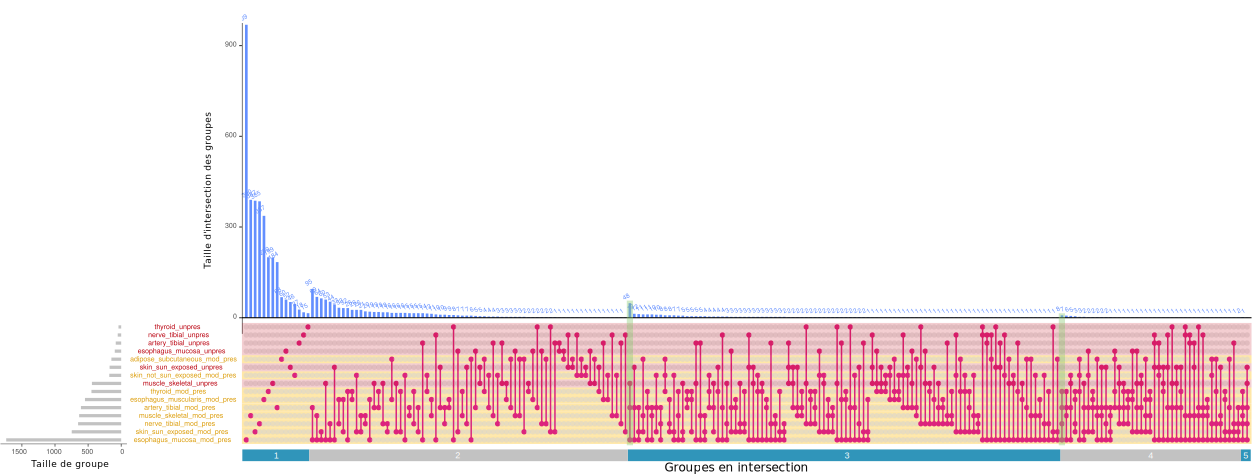
\includegraphics[width=1\textheight]{img/chap2/chap2_upset_genes_unpres_modpres_by_tissue.pdf}
    \end{adjustbox}
    \label{figure:upset_intersection_genes_tissu_unpres_modpres}
\end{figure}


Comme suggéré par les ratios de statut de préservation en table \ref{table:modules_status_all_tissues}, certains tissus tendent à avoir plus de modules MP/NP et/ou des modules de plus grande taille (avec le plus de gènes), favorisant alors leur probabilité de recoupement avec d'autres tissus. Ainsi, les modules MP de la muqueuse œsophagienne regroupent 1750 gènes et tendent à se positionner dans plus d'intersection que la moyenne. Une séparation est toutefois visible entre les deux types de statut MP et NP dans les intersection au delà de 2 tissus et avec un minimum de trois gènes.

\subsection{Répartition des phénomènes communs liés au vieillissement dans plusieurs tissus}

Pour mieux comprendre les fonctions physiologiques communes en jeu et pouvant être impliquées dans le vieillissement, les intersections de plus de 3 tissus et ayant au moins 5 gènes on été enrichies via GWENA. Comme visible en Annexe \ref{annexe:chap_2_genes_intersect_enrichments} dans les tables des enrichissements obtenus, 5 intersections n'ont pas donné d'enrichissement significatif malgré un nombre de gène équivalent à d'autres intersections avec enrichissement. Les 18 autres intersections ont quant à elles retourné des fonctions physiologiques (Gene Ontology \cite{Ashburner2000}, CORUM \cite{Ruepp2008}) et voies d'activation (KEGG \cite{Kanehisa2019}, REACTOME \cite{Fabregat2016}, WikiPathways\cite{Slenter2018}) connues comme faisant partie du vieillissement global, ou de manifestations spécifiques à plusieurs tissus. Ainsi on retrouve, dans ces intersections de modules peu ou pas préservés dans la tranche âgée, des fonctions associées à l'homéostasie, la régulation de la transcription, la gestion des dérivés réactifs de l'oxygène, l'inflammation, etc. (Table \ref{table:intersection_aging_global_phenomenons} et Figure \ref{figure:revigo_resume_4_enrich}). La muqueuse œsophagienne bien qu'ayant un nombre de gènes plus élevé que les autres tissus ne se retrouve pas sur-représentée dans ces phénomènes observés. Cela indique donc que la majorité de ses gènes se trouvent dans les intersections de faible taille, tant en gènes qu'en nombre de tissus recoupés. Le sang complet, le tissu adipeux sous-cutané, et la peau non exposée au soleil sont eux les tissus les moins présents dans ces intersections avec des phénomènes liés au vieillissement. Le sang complet est notablement absent des intersection avec des phénomènes liés à la coagulation. Les tissus ayant un fort renouvellement (voir en partie \ref{tissu_telomere_effet}) que sont les épithéliums (peau exposée au soleil, artère tibiale, muqueuse œsophagienne) sont porteurs d'un grand nombre de phénomènes, ainsi que la thyroïde et le muscle squelettique. 


\begin{table}[]
\resizebox{\textwidth}{!}{
\begin{tabular}{@{}lllllllllll@{}}
\rotatebox{90}{\textbf{Muqueuse œusophagienne}}   & \rotatebox{90}{\textbf{Artère tibiale}}                      & \rotatebox{90}{\textbf{Thyroïde}}                 & \rotatebox{90}{\textbf{Muscle squelettique}}      & \rotatebox{90}{\textbf{Peau exposée au soleil}}   & \rotatebox{90}{\textbf{Muscle œusophagien}}       & \rotatebox{90}{\textbf{Nerf tibial}}              & \rotatebox{90}{\textbf{Peau non exposée au soleil}} & \rotatebox{90}{\textbf{Adipeux sous-cutané}}      & \rotatebox{90}{\textbf{Sang complet}}             & \textbf{Phénomène du vieillissement observé}       \\ \midrule
\cellcolor[HTML]{F8A102} & \cellcolor[HTML]{F8A102}            &                          & \cellcolor[HTML]{F8A102} &                          &                          &                          & \cellcolor[HTML]{F8A102}   &                          &                          & Homéostasie                               \\
                         & \cellcolor[HTML]{F8A102}            & \cellcolor[HTML]{F8A102} &                          &                          & \cellcolor[HTML]{F8A102} &                          &                            &                          &                          & Régulation de la transcription            \\
\cellcolor[HTML]{F8A102} &                                     & \cellcolor[HTML]{F8A102} & \cellcolor[HTML]{F8A102} &                          &                          &                          &                            &                          &                          & Dérivés réactifs de l'oxygène - peroxydes \\
                         &                                     & \cellcolor[HTML]{F8A102} &                          & \cellcolor[HTML]{F8A102} & \cellcolor[HTML]{F8A102} & \cellcolor[HTML]{F8A102} &                            &                          &                          & Dérivés réactifs de l'oxygène - dGTP      \\
                         &                                     & \cellcolor[HTML]{F8A102} &                          &                          &                          &                          & \cellcolor[HTML]{F8A102}   & \cellcolor[HTML]{F8A102} &                          & Inflammation                              \\
                         &                                     &                          &                          & \cellcolor[HTML]{F8A102} & \cellcolor[HTML]{F8A102} & \cellcolor[HTML]{F8A102} &                            &                          &                          & Désamination                              \\
\cellcolor[HTML]{F8A102} & \cellcolor[HTML]{F8A102}            &                          &                          &                          &                          & \cellcolor[HTML]{F8A102} &                            &                          &                          & Coagulation - plaquettes                  \\
\cellcolor[HTML]{F8A102} & \cellcolor[HTML]{F8A102}            & \cellcolor[HTML]{F8A102} &                          &                          &                          & \cellcolor[HTML]{F8A102} &                            &                          &                          & Coagulation - global                      \\
\cellcolor[HTML]{F8A102} & \cellcolor[HTML]{F8A102}            &                          & \cellcolor[HTML]{F8A102} &                          &                          &                          &                            &                          &                          & Méthylation - folate, B12, selenium       \\
                         &                                     &                          & \cellcolor[HTML]{F8A102} & \cellcolor[HTML]{F8A102} &                          &                          &                            & \cellcolor[HTML]{F8A102} &                          & Méthylation - déméthylase                 \\
\cellcolor[HTML]{F8A102} & \cellcolor[HTML]{F8A102}            &                          & \cellcolor[HTML]{F8A102} &                          &                          &                          &                            &                          & \cellcolor[HTML]{F8A102} & Altération de la MEC                      \\
                         &                                     & \cellcolor[HTML]{F8A102} &                          & \cellcolor[HTML]{F8A102} & \cellcolor[HTML]{F8A102} &                          &                            &                          &                          & Anomalie du taux de glutamine             \\
\cellcolor[HTML]{F8A102} &                                     &                          &                          & \cellcolor[HTML]{F8A102} &                          &                          & \cellcolor[HTML]{F8A102}   &                          &                          & Synthèse de pigment (dont mélanine)      \\
\cellcolor[HTML]{F8A102} & \cellcolor[HTML]{F8A102}            & \cellcolor[HTML]{F8A102} & \cellcolor[HTML]{F8A102} &                          &                          &                          &                            &                          &                          & Anomalie du taux de fer                   \\
\midrule
8                        & 7                                   & 7                        & 6                        & 5                        & 4                        & 4                        & 3                          & 2                        & 1                        & \textbf{Total}                   
\end{tabular}
}
\caption{Phénomènes connus dans le vieillissement et observés dans les intersections de modules MP et NP pour chaque tissu. Les modules MP et NP ont été joints par tissus et les tissus ont été ordonnés par nombre décroissant de phénomènes du vieillissement présent. MEC : Matrice extra-cellulaire.}
\label{table:intersection_aging_global_phenomenons}
\end{table}

% \begin{table}[]
% \resizebox{\textwidth}{!}{
% \begin{tabular}{@{}lllllllllll@{}}
% % \toprule
% \rotatebox{90}{\textbf{Adipeux sous-cutané }}      & \rotatebox{90}{\textbf{Artère tibiale }}           & \rotatebox{90}{\textbf{Muqueuse œusophagienne }}   & \rotatebox{90}{\textbf{Muscle œusophagien }}       & \rotatebox{90}{\textbf{Muscle squelettique }}      & \rotatebox{90}{\textbf{Nerf tibial }}              & \rotatebox{90}{\textbf{Peau non exposée au soleil }} & \rotatebox{90}{\textbf{Peau exposée au soleil }}   & \rotatebox{90}{\textbf{Thyroïde }}                 & \rotatebox{90}{\textbf{Sang complet }}             & \textbf{Phénomène du vieillissement observé}       \\ \midrule
%                          & \cellcolor[HTML]{F8A102} & \cellcolor[HTML]{F8A102} &                          & \cellcolor[HTML]{F8A102} &                          & \cellcolor[HTML]{F8A102}   &                          &                          &                          & Homéostasie                               \\
%                          & \cellcolor[HTML]{F8A102} &                          & \cellcolor[HTML]{F8A102} &                          &                          &                            &                          & \cellcolor[HTML]{F8A102} &                          & Régulation de la transcription            \\
%                          &                          & \cellcolor[HTML]{F8A102} &                          & \cellcolor[HTML]{F8A102} &                          &                            &                          & \cellcolor[HTML]{F8A102} &                          & Dérivés réactifs de l'oxygène - peroxydes \\
%                          &                          &                          & \cellcolor[HTML]{F8A102} &                          & \cellcolor[HTML]{F8A102} &                            & \cellcolor[HTML]{F8A102} & \cellcolor[HTML]{F8A102} &                          & Dérivés réactifs de l'oxygène - dGTP      \\
% \cellcolor[HTML]{F8A102} &                          &                          &                          &                          &                          & \cellcolor[HTML]{F8A102}   &                          & \cellcolor[HTML]{F8A102} &                          & Inflammation                              \\
%                          &                          &                          & \cellcolor[HTML]{F8A102} &                          & \cellcolor[HTML]{F8A102} &                            & \cellcolor[HTML]{F8A102} &                          &                          & Désamination                              \\
%                          & \cellcolor[HTML]{F8A102} & \cellcolor[HTML]{F8A102} &                          &                          & \cellcolor[HTML]{F8A102} &                            &                          &                          &                          & Coagulation - plaquettes                  \\
%                          & \cellcolor[HTML]{F8A102} & \cellcolor[HTML]{F8A102} &                          &                          & \cellcolor[HTML]{F8A102} &                            &                          & \cellcolor[HTML]{F8A102} &                          & Coagulation - global                      \\
%                          & \cellcolor[HTML]{F8A102} & \cellcolor[HTML]{F8A102} &                          & \cellcolor[HTML]{F8A102} &                          &                            &                          &                          &                          & Méthylation - folate, B12, selenium       \\
% \cellcolor[HTML]{F8A102} &                          &                          &                          & \cellcolor[HTML]{F8A102} &                          &                            & \cellcolor[HTML]{F8A102} &                          &                          & Méthylation - déméthylase                 \\
%                          & \cellcolor[HTML]{F8A102} & \cellcolor[HTML]{F8A102} &                          & \cellcolor[HTML]{F8A102} &                          &                            &                          &                          & \cellcolor[HTML]{F8A102} & Altération de la MEC                      \\
%                          &                          &                          & \cellcolor[HTML]{F8A102} &                          &                          &                            & \cellcolor[HTML]{F8A102} & \cellcolor[HTML]{F8A102} &                          & Anomalie du taux de glutamine             \\
%                          &                          & \cellcolor[HTML]{F8A102} &                          &                          &                          & \cellcolor[HTML]{F8A102}   & \cellcolor[HTML]{F8A102} &                          &                          & Synthèse de pigement (dont mélanine)      \\
%                          & \cellcolor[HTML]{F8A102} & \cellcolor[HTML]{F8A102} &                          & \cellcolor[HTML]{F8A102} &                          &                            &                          & \cellcolor[HTML]{F8A102} &                          & Anomalie du taux de fer                   \\ 
% \end{tabular}
% }
% \caption{Phénomènes connus dans le vieillissement et observés dans les intersections de modules MP et NP pour chaque tissu. Les modules MP et NP ont été joints par tissus pour une meilleure lisibilité.}
% \label{table:intersection_aging_global_phenomenons}
% \end{table}

\begin{figure}
    \centering
    \includegraphics[width=1\textwidth]{img/chap2/chap2_revigo_resume_4_enrich.png}
    \caption{Exemple de résumé des enrichissements sur GO pour 4 des intersections par carte proportionnelle. Chaque ensemble de GO terme partageant une ontologie parente commune (selon un score de similarité) est groupé sous une même couleur. Chaque carte présente ici un phénomène connu dans le vieillissement : A. Homéostasie (GO *Biological Process*), B. Régulation de la transcription (GO *Biological Process*), C. Dérivés réactifs de l'oxygène (GO *Molecular Function*), D. Inflammation (GO *Biological Process*) }
    \label{figure:revigo_resume_4_enrich}
\end{figure}

Des anomalies phénotypiques ont été relevée (via enrichissement sur HPO \cite{Kohler2019}) et présentent un lien plus ou moins évident avec les altérations physiologiques précédemment relevées. Aux anomalies du taux de fer détectés dans les fonctions physiologiques coïncident ainsi des phénotypes d'anémie (déficience en taux de globules rouges ou en concentration d'hémoglobine) ou de défaut de coagulation avec hémorragies diverses (epistaxie, saignement gingival, menstruations hors cycle, hémoragie cérébrale). De même, les tissus présentant une altération de la matrice extra-cellulaire (MEC) ont été associés avec des taux élevés de protéine C-réactive et d'anomalies de la fonction exocrine du pancréas ainsi que de malabsorption des lipides et ce qui en découle (stéatorrhée, pancréatite, thrombose veineuse). Ces résultats confirment le lien entre vieillissement et dérèglement progressif de l'homeostasie entrainant en cascade des pathologies de trouble de la coagulation \cite{Franchini2006,Kario1993} et de la dégradation des lipides circulants \cite{Yamamoto2014, Hirschfield2003}. Cependant d'autres résultats semblent moins intuitifs comme dans le cas de pathologies liées au sexe (azoospermie, maladie d'hérédité gonosomale) relevées parallèlement à la déméthylation dans le tissu adipeux, le muscle squelettique, et la peau non exposée au soleil. Ces informations, en l'absence d'erreur technique, semblent continuer de montrer la complexité des relations entre pathologies et vieillissement.

Enfin, on a exploré le vieillissement et son phénomène de perturbation de la régulation de la transcription en évaluant l'enrichissement d'éléments de régulation (MiRTarBase \cite{Chou2018}, TRANSFAC \cite{Matys2006}). L'intersection présentant des phénomènes de coagulation globale est ainsi fortement enrichi en micro ARN (miARN). Ceux contiennent notamment des miARN associés aux 3 gènes de la génération de fibrinogène FGA, FGB, FGG comme détectés lors du chapitre précédent. Quelques autres intersections. Deux facteurs de transcription (FT), HNF1A et HNF1B, sont également significatifs bien que normalement exprimés dans le foie. Cela s'explique par la production de facteurs de la coagulation (dont FGA, FGB, FGG) dans celui-ci et un effet connu de l'altération de production de ces facteurs dans le cadre d'une perturbation de l'expression de HNF1A et HNF1B \cite{Costa2003}. L'intersection associée à l'inflammation quand a elle ne présente qu'un seul miARN agissant ici sur RSAD2, IFI44, OASL, et EPSTI1 présents dans l'intersection. RSAD2 et OASL sont également connus pour être stimulé par des interférons de classe I (\textalpha et \textbeta) qui ont entre autres IRF1 (pour interferon related factor 1) pour FT \cite{Schoggins2011}. Ce facteur IRF1 fait par ailleurs parti de la liste des FT détectés dans cette intersection. On y trouve un large panel d'autres membres de la famille d'IRF (de 1 à 9 à l'exception d'IRF6) dont l'implication dans l'inflammation s'exerce tant dans la réaction innée que acquise \cite{Frisch2020}. Mais tous les FT détectés via enrichissement n'étaient pas des IRF. Bien que n'étant pas directement liés à la régulation des interférons, STAT2 est présent dans la voie de signalisation des interférons \textalpha et \textbeta détecté plus tôt (R-HSA-909733). Le dernier FT identifié, FOXP1, n'est quant à lui pas contenu dans cette voie mais agit sur l'engagement des cellules souches mésenchymateuses et la sénescence au cours du vieillissement \cite{Infante2018} et sur de la régulations d'autres cytokines, l'interleukine 1 et 12 d'après UniprotKB (Q9H334).

\subsection{Les variation de co-expression dans l'intersection liée à l'inflammation}

L'inflammation systémique chronique de faible intensité est une des marques connues du vieillissement \cite{Lopez-Otin2013, Franchini2006}. La complexité des mécanismes d'immunité et d'inflammation rend ce phénomène particulièrement difficile à étudier et les publications actuelles tendent donc à cibler un ou quelques acteurs afin de 
% L'inflammation systémique chronique de faible intensité est une manifestation courante du vieillissement.
% La détection de ces différents phénomènes liée à l'âge ayant été permise par le ciblage 

\begin{figure}[b]
    \centering
    \includegraphics[width=1\textwidth]{img/chap2/chap2_graphs_intersection_plot_adipo_skinnosun_thyr.png}
    \caption{Réseaux de co-expression des gènes de l'intersection associée au phénomène d'inflammation lors du vieillissement entre les deux tranches d'âge. Le réseau est filtré à 0.95 de dissimilarité (sur une échelle de 0 à 1) et 3 tissus sont présentés : tissu adipeux, peau non exposée au soleil, et thyroïde.}
    \label{figure:graphs_intersection_plot_adipo_skinnosun_thyr}
\end{figure}



\subsection{Cas particulier : le vieillissement spécifique à la peau}



\subsection{Variation de la co-expression dans le XXX}
Comme attendu au vu de la littérature, de nombreux enrichissements ont retourné des mécanismes et acteurs de l'inflammation. 




\#\#\#\#\#\#\#\#\#\#\#\#\# TRAVAIL EN COURS \#\#\#\#\#\#\#\#\#\#\#\#\#


% Pourquoi le muscle vieillit vite malgré son faible taux de renouvellement : https://www.ncbi.nlm.nih.gov/pmc/articles/PMC3874224/

% À l'inverse, certains gènes dans les modules MP ou NP ne sont présent que dans leur tissu. Ceux-ci pouvant témoigner de fonctions physiologiques propres au vieillissement de ces tissus, ils ont également été enrichis module par module.

% Les origines de la faible ou non préservation liées au vieillissement pouvant être variées, on a souhaité étudier les fonctions physiologiques contenues dans ces modules non préservés et peu préservés.

% # Graphes de qques modules d'intérêt
% Tests de diminution de co-expression 


\section{Discussion}

% 10.1371/journal.pcbi.1004220 p4 pour discuter la proximité des tissus
% https://thyroidresearchjournal.biomedcentral.com/articles/10.1186/1756-6614-5-16 pour expliquer la faible connaissance du fonctionnement/effet de la thyroide dans le vieillissement malgré son affectation par masse de de phénomènes du vieillissement \ref{table:intersection_aging_global_phenomenons}
% Explication potentielle du pourquoi une reaction virale alors que pas de virus : https://www.nature.com/articles/s41586-018-0784-9 + https://link.springer.com/chapter/10.1007/978-3-319-48344-3_13


\section{Conclusion}








% ##############################################################################

% Idées initiales de chapitre 2 - abandonnées :
% \begin{itemize}
%     \item Rajout d'information protéique pour "consolider" le réseau ?
%     \item Rajout d'une méthode de réseau consensus à GWENA ?
%     \item Differential co-expression avec un autre tissu sur lequel on peut avoir des jeux de données jeune/vieux pour récup les genes communs au vieillissement, ceux specifique à un tissu ou l'autres, et ceu combinant le vieillissement specifique au tissu ?
%     \item Une étude de l'impacte de la filtration sur l'état du réseau final ? Il n'y a rien de systemique dans la littérature, personne qui en fasse une review. Parsana et al. (alexis battle team) a fait ça en 2019 pour tester la PC-correction uniquement. Ils ont simulé des données scale free + des données scale free mimiquant GTEx et essayé de déterminer l'impact en calculant un FDR
% \end{itemize}    % chapitre 2, etc.
\chapter*{Conclusion}         % ne pas numéroter
\phantomsection\addcontentsline{toc}{chapter}{Conclusion} % dans TdM


Après avoir présenté une vue d'ensemble des technologies de transcriptomique et leur intérêt dans la recherche en médecine moléculaire, cette thèse s'est attardée sur une présentation détaillée de l'analyse par réseaux de co-expression de gènes. Les méthodes de préparation des données, de construction du réseau, de détection des modules et leur exploitation avec ou sans connaissance a priori ont été examinées par rapport aux connaissances dans la littérature actuelle. Chaque étape demandant un niveau de maîtrise poussé en biostatistique ou théorie des graphes, il était important d'expliciter chacun des choix fait pour mieux comprendre la démarche poursuivie durant ce doctorat. 
L'adéquation de l'analyse par réseaux de co-expression de gènes pour l'étude du vieillissement a ensuite été mise en avant après une présentation concise du vieillissement, de ses manifestations cellulaire et moléculaire, ainsi que les enjeux qu'il représente.

Face à la difficulté d'emploi des outils existant sans expertise, la pénibilité de leur combinaison et de la faible pérennité d'une analyse avec les outils actuels pour réaliser une analyse par réseaux de co-expression de gènes, on avait formulé une première hypothèse qui s'interrogeait sur la faisabilité d'un outil pipeline sous la forme d'un progiciel R déposé sur Bioconductor pour répondre à ces problèmes. Grâce au développement du progiciel GWENA présenté en \hyperref[chapter:gwena]{Chapitre 1} on a démontré qu'il était possible d'avoir un outil facilitant l'analyse par réseaux de co-expression de gènes de bout en bout et qui, grâce à une architecture modulaire, était voué à s'adapter aux dernières avancées méthodologiques sur ce type d'analyse. Avec une étude de cas dédiée au vieillissement du muscle, il a également été possible de montrer la valeur ajoutée de la co-expression différentielle dans la priorisation de gènes d'une condition donnée. L'analyse de topologie a elle permit de venir préciser un phénomène déjà observé chez la souris mais pas encore chez l'homme à ce jour : une déconnexion modulaire de gènes dans le réseaux avec le vieillissement. Mieux encore, il a été mis en évidence que cette déconnexion modulaire s'accompagnait d'une reconnexion centralisée autour des gènes pivots dans le réseau.

Fort de cette capacité de GWENA à innover dans la recherche sur le vieillissement, la seconde hypothèse supposait qu'il serait à même de trouver de nouveaux gènes candidats par co-expression différentielle non pas simplement entre deux tranches d'âge, mais en plus à travers plusieurs tissus. Le \hyperref[chapter:multidim]{Chapitre 2} présente donc l'utilisation des différents outils intégrés à GWENA pour réaliser une analyse parallélisée de couples tissu et tranche d'âge. L'identification parmi les modules modérément ou non préservés de nombreux phénomènes du vieillissement tels qu'énoncés dans les marques principales du vieillissement établies par López-Otín \textit{et al.} a permit de valider la démarche de co-expression différentielle et d'aller plus en avant dans l'exploitation de ces modules. Par un recoupement des gènes contenus dans chacun des modules, des gènes impliqués dans des phénomènes du vieillissement spécifiques à quelques tissus ou à l'inverse commun à la majorité ont été détectés. Une analyse topologique faite dans un exemple de gènes spécifiques et un exemple de gènes communs a finalement retourné de nouveaux gènes pertinents dans la compréhension du vieillissement au vu des annotations dont ils bénéficiaient déjà.

Chacun de ces chapitres aura donc, en plus de montrer l'intérêt de GWENA, permis de détecter de nouveaux gènes candidats au vieillissement humain. Ceux-ci devront à l'avenir faire l'objet de validation expérimentale.

            % conclusion
\setcounter{chapter}{5}
\setcounter{section}{0}
\setcounter{figure}{0}   
\chapter*{Discussion}         % ne pas numéroter
\phantomsection\addcontentsline{toc}{chapter}{Discussion} % dans TdM

\section{L'apport de mes travaux sur l'étude du vieillissement}

\begin{itemize}
    \item La création d'un outil de type pipeline avec comparison et analyse intégrée
    \item La démonstration de son application chez le muscle et le ciblage de gènes potentiellements liés au vieillissement
    \item whatever secodn article
    \item Les études de quantification de l'expression c'est bien, mais grâce au RNA-seq on peut aller explorer d'autres pan du transcriptome et potentiellement faire des recoupements avec des phénomènes/mécanismes observés via quantification de l'expression
\end{itemize}

\section{Analyse critique}
% \section{limitations}
\begin{itemize}
    \item De nombreux jeux de données de puces à ADN et RNA-seq sont disponibles sur GEO et ArrayExpress sans jamais avoir été analysés par réseau de co-expression. Encore moins d'entre eux ont étés analysés par co-expression différentielle alors que plusieurs conditions sont souvent disponible vu qu'une analyse classique d'expression différentielle est régulièrement effectuée. Ces jeux de données représentent un potentiel de connaissance non exploitée et peuvent également servir d'étude préalable à l'investigation d'une maladie, d'un phénotype, ou plus généralement d'une hypothèse. % http://journal.frontiersin.org/Article/10.3389/fpls.2016.00444/abstract
    \item Les réseaux de co-experssion se basant sur l'assomption d'un réseau invariant d'échelle ne sont justes mais une autre loi que celle de puissance peut Être fittée souvent (https://www.nature.com/articles/s41467-019-08746-5)
    \item Les réseaux de co-expression comme moyen d'étude mais de nouvelles méthodes moins bruitée se mettent en place %% https://www.nature.com/articles/s42255-020-00304-4 et https://www.nature.com/articles/s42255-020-00295-2 (pas un article mais un News and Views qui resume)
    \item Ne permettent pas directement de connaitre le sens de régulation, il faut d'autres analyses pour inférer le sens de la relation dans un réseau de co-expression. Avec ça vient les soucis d'inférence évoqués par marie laure : co-regulation, manque de puissance stat..
    \item D'autres outils que WGCNA existent, pourquoi lui ? Pourquoi pas ARACNE ? (https://journals.plos.org/plosone/article?id=10.1371/journal.pone.0029348). WGCNA ne permet pas de chevauchement des modules, hors on sait que les gènes sont impliqués dans plusieurs pathways et ça serait d'autant plus intéressant vu les résultats qu'on a obtenus dans le chapitre 1 où on montre un switch de fonctionnalité.
\end{itemize}



\section{Perspectives}

- la potentielle application dans l'étude du cancer ou dans une étude comparative concernant la perte de connectivité observée là bas également 10.1371/journal.pone.0087075
- l'utilisation dans des populations d'ethinies plus minoritaires, malheureusement les données et bdd sont faibles par rapport à la puissance stat requise
- L'analyse en time-course et co-expression différentielle permettrait une analyse plus fine des variations de mécanismes cellulaires en réponse à un stress aigu ou une croissance. % http://journal.frontiersin.org/Article/10.3389/fpls.2016.00444/abstract
- Il existe d'autres types de réseaux complémentaires "A very clear partition of different biological networks is provided by Christensen et al. [1], who separated these networks into five main categories as follows :" cf https://academic.oup.com/bfg/article-lookup/doi/10.1093/bfgp/elt003
- approches multi-omiques avec intégration de réseaux protein-protein % <- ptet plus dans mise en contexte des travaux            % discussion


\bibliographystyle{plain-fr}    % bibliographie
\bibliography{bibliographie}    % nom du fichier .bib

% \appendix                       % annexes le cas échéant
% \chapter*{Annexes}
% \addcontentsline{toc}{chapter}{Annexes}
% \chapter{Questions en bio-informatique}

Cette annexe a pour vocation de regrouper les nombreuses questions qui ont pu se poser durant cette thèse. Bien que parfois basiques, elles n'en sont pas moins légitimes. Beaucoup de ces questions on vu leur réponse plus longue que prévu à trouver en raison de consensus installés dans la communauté, de reflex de chercheur, etc. sans savoir l'origine de ceux-ci.

\section{Pourquoi normalisation log2 pour le microarray ?}
Le log pour passer à une échelle symétrique autour de 0, le 2 car c'est + facile à interpréter, chaque fois qu'on augmente le ratio Ti de 1, on double la up regulation 
%% (https://www.researchgate.net/post/Why_do_we_usually_use_Log2_when_normalizing_the_expression_of_genes et https://www.nature.com/articles/ng1032z)

      % annexe
% \chapter{NetRep statistics detail}


\todo{TODO : récupérer, résumer (et traduire ?) l'explication et l'interprétation biologique des 7 métriques disponibles dans les Supplemental Experimental Procedures de la publication de netrep (https://doi.org/10.1016/j.cels.2016.06.012)}

Source : Document S1. Supplemental Experimental Procedures, Figures S1–S7, and Tables S1–S4, S6, and S7 from 

% \chapter{Demande d'accès dbGaP aux données protégées de GTEx}
\label{annexe:dbgap}

\section{Query title}
Muscle gene co-expression in multiple age range for sarcopenia condition exploration

\section{Research use statement}
As a multi factorial phenomena, aging is a complex condition to study. Current analysis of transcriptomic data joined with phenotypic ones have unravel few genes and environmental variables impacting it. However, aging remains not fully understood. These may come from current approaches focusing on single factors while aging is more about interaction between many of them. This is why we would like to study it through the spectrum of the co-expression networks. However, because aging is already complex by itself, we will focus on a single tissue in the beginning : muscle. Reasons are myopenia and dynapenia (known together as sarcopenia) are responsible for loss of autonomy, weak metabolic aggression resistance, and increased mortality.
By using our yet to be published pipeline developed in our lab, we aim to build gene co-expression modules and network from transcriptomic data and characterize them with external resources. This pipeline begin with a quality assessment of the data, based on the technique used to get transcriptomic information (either microarray or RNA-Seq). It then compute co-expression levels and detects modules by using the WGCNA package. Additionnal steps are then performed to fully charachterize the modules : biological enrichment, topological study, phenotipic association, differentially expressed and condition-specific gene positionning.The external resources used to it include : enrichment databases (GO, KEGG, etc.), phenotypic information (exact age, condition of death, ethnicity), and age related databases (Digital aging atlas, Aging map, etc.). The use of these complementary information represents no additional risk to participants since only summarized gene information we'll be used in the form of modules. No other raw transcriptomics data will be combined to the GTEx data, but only a comparison of the modules built on each datasets in order to study the reproductibility of our modules, and the comparison with modules built on sarcopenia dedicated datasets.
Phenotipyc information is the main reason for our current demand regarding protected datasets because we think precise age and cause of death will impact the aging expression. 
No collaboration with other institution is planned.
Finnally, this methodological work will advance the understanding of the genetic bases of the aging processes occurring in the muscle.


\section{Non-technical summary}
Aging affect every one of us. It is defined as the progressive degradation of biological functions inside the body. In the muscle, this results in a decreasing in muscle density and strength called sarcopenia. They are responsible for mobility difficulties, therefore autonomy, and a deficit in body protection against aggression, sometimes leading to death. With this risks at stake, it is understandable that a better understanding of aging processes in muscle is important for public health. Few single genes linked to it have already been discovered, however we still don't fully understand the mechanisms occurring and how to limit them. Gene expression is a witness of the changes in the body mechanisms. By studying the expression of the genes and the coordination between this levels of expression, therefore patterns of expression, we aim to detect news genes involved in muscle aging. Do to so, we regroup the most coordinated genes in entities called module and try to unravel the biological interactions which link them. Because some of this genes are already involved into other biological interactions, we can have an insight on the regulations that take place in this case by extrapolating information. These, will lead to the discovery of new genes associated with sarcopenia.

\hfill \break
\textit{Réalisé le 30/09/2019}

\textcolor[RGB]{220,220,220}{\rule{\linewidth}{0.2pt}}

\section{Access update : Research Progress}
Current analysis of the GTEx data focused on the skeletal muscle samples as we are studying sarcopenia and other aging impact on muscle. The RNAseq data was then split in two opposite age range (young and old) to emphase and capture the differences in aging through our newly developped differential gene co-expression network pipeline GWENA (\url{https://www.bioconductor.org/packages/release/bioc/html/GWENA.html}). 
A first analysis solely on the modules (gene groups) detected by GWENA in the young condition. A selection of interesting modules for muscle activity was achieved through a combinaison of moduels phenotypic association and gene sets enrichment. Inside one promissing module, hub genes connected in the network to genes involved in muscle activity allowed the identification of genes with strong evidence of contribution to muscle developpemnt and growth.
A second analysis used the full potential of the differential co-expression analysis offered by GWENA to find specific co-expression modules to aging. Important topological variation lead us to focus on one module. Further investigation is currently underway to characterise the origin of the specificity and this variations. 

\hfill \break
\textit{Réalisé le 01/12/2020}

\renewcommand{\appendixpagename}{Annexes}
\renewcommand{\appendixtocname}{Annexes}
\appendixpage
\begin{appendices}
    \chapter{Questions en bio-informatique}

Cette annexe a pour vocation de regrouper les nombreuses questions qui ont pu se poser durant cette thèse. Bien que parfois basiques, elles n'en sont pas moins légitimes. Beaucoup de ces questions on vu leur réponse plus longue que prévu à trouver en raison de consensus installés dans la communauté, de reflex de chercheur, etc. sans savoir l'origine de ceux-ci.

\section{Pourquoi normalisation log2 pour le microarray ?}
Le log pour passer à une échelle symétrique autour de 0, le 2 car c'est + facile à interpréter, chaque fois qu'on augmente le ratio Ti de 1, on double la up regulation 
%% (https://www.researchgate.net/post/Why_do_we_usually_use_Log2_when_normalizing_the_expression_of_genes et https://www.nature.com/articles/ng1032z)


    \chapter{NetRep statistics detail}


\todo{TODO : récupérer, résumer (et traduire ?) l'explication et l'interprétation biologique des 7 métriques disponibles dans les Supplemental Experimental Procedures de la publication de netrep (https://doi.org/10.1016/j.cels.2016.06.012)}

Source : Document S1. Supplemental Experimental Procedures, Figures S1–S7, and Tables S1–S4, S6, and S7 from 

    \chapter{Demande d'accès dbGaP aux données protégées de GTEx}
\label{annexe:dbgap}

\section{Query title}
Muscle gene co-expression in multiple age range for sarcopenia condition exploration

\section{Research use statement}
As a multi factorial phenomena, aging is a complex condition to study. Current analysis of transcriptomic data joined with phenotypic ones have unravel few genes and environmental variables impacting it. However, aging remains not fully understood. These may come from current approaches focusing on single factors while aging is more about interaction between many of them. This is why we would like to study it through the spectrum of the co-expression networks. However, because aging is already complex by itself, we will focus on a single tissue in the beginning : muscle. Reasons are myopenia and dynapenia (known together as sarcopenia) are responsible for loss of autonomy, weak metabolic aggression resistance, and increased mortality.
By using our yet to be published pipeline developed in our lab, we aim to build gene co-expression modules and network from transcriptomic data and characterize them with external resources. This pipeline begin with a quality assessment of the data, based on the technique used to get transcriptomic information (either microarray or RNA-Seq). It then compute co-expression levels and detects modules by using the WGCNA package. Additionnal steps are then performed to fully charachterize the modules : biological enrichment, topological study, phenotipic association, differentially expressed and condition-specific gene positionning.The external resources used to it include : enrichment databases (GO, KEGG, etc.), phenotypic information (exact age, condition of death, ethnicity), and age related databases (Digital aging atlas, Aging map, etc.). The use of these complementary information represents no additional risk to participants since only summarized gene information we'll be used in the form of modules. No other raw transcriptomics data will be combined to the GTEx data, but only a comparison of the modules built on each datasets in order to study the reproductibility of our modules, and the comparison with modules built on sarcopenia dedicated datasets.
Phenotipyc information is the main reason for our current demand regarding protected datasets because we think precise age and cause of death will impact the aging expression. 
No collaboration with other institution is planned.
Finnally, this methodological work will advance the understanding of the genetic bases of the aging processes occurring in the muscle.


\section{Non-technical summary}
Aging affect every one of us. It is defined as the progressive degradation of biological functions inside the body. In the muscle, this results in a decreasing in muscle density and strength called sarcopenia. They are responsible for mobility difficulties, therefore autonomy, and a deficit in body protection against aggression, sometimes leading to death. With this risks at stake, it is understandable that a better understanding of aging processes in muscle is important for public health. Few single genes linked to it have already been discovered, however we still don't fully understand the mechanisms occurring and how to limit them. Gene expression is a witness of the changes in the body mechanisms. By studying the expression of the genes and the coordination between this levels of expression, therefore patterns of expression, we aim to detect news genes involved in muscle aging. Do to so, we regroup the most coordinated genes in entities called module and try to unravel the biological interactions which link them. Because some of this genes are already involved into other biological interactions, we can have an insight on the regulations that take place in this case by extrapolating information. These, will lead to the discovery of new genes associated with sarcopenia.

\hfill \break
\textit{Réalisé le 30/09/2019}

\textcolor[RGB]{220,220,220}{\rule{\linewidth}{0.2pt}}

\section{Access update : Research Progress}
Current analysis of the GTEx data focused on the skeletal muscle samples as we are studying sarcopenia and other aging impact on muscle. The RNAseq data was then split in two opposite age range (young and old) to emphase and capture the differences in aging through our newly developped differential gene co-expression network pipeline GWENA (\url{https://www.bioconductor.org/packages/release/bioc/html/GWENA.html}). 
A first analysis solely on the modules (gene groups) detected by GWENA in the young condition. A selection of interesting modules for muscle activity was achieved through a combinaison of moduels phenotypic association and gene sets enrichment. Inside one promissing module, hub genes connected in the network to genes involved in muscle activity allowed the identification of genes with strong evidence of contribution to muscle developpemnt and growth.
A second analysis used the full potential of the differential co-expression analysis offered by GWENA to find specific co-expression modules to aging. Important topological variation lead us to focus on one module. Further investigation is currently underway to characterise the origin of the specificity and this variations. 

\hfill \break
\textit{Réalisé le 01/12/2020}
\end{appendices}


% \chapter*{Glossaire}                                        % enlève la numérotation
\phantomsection\addcontentsline{toc}{chapter}{Glossaire}    % inclus le glossaire dans la table des matières

\printglossary[nonumberlist]
% \glsaddall

\footnotetext{Les définitions précédées d'un [W] sont issues de Wikipédia}

%% MODELE

%\newglossaryentry{}
%{
%	name={},
%	description={}, 
%	plural={}
%}



\newglossaryentry{}
{
	name={},
	description={}, 
	plural={}
}

\newglossaryentry{transcrit}
{
	name={transcrit},
	description={version d'ARN messager issue d'un gène}, 
	plural={transcrits}
}

\newglossaryentry{aging_hallmarks}
{
	name={marque principale},
	description={représentation des causes et conséquence du vieillissement en neuf marques réalisée par López-Otín \cite{Lopez-Otin2013}}, 
	plural={marques principales}
}

\newglossaryentry{plus_court_chemin}
{
	name={plus court chemin},
	description={suite de liens d'un nœud à un autre de longueur la plus petite possible}, 
	plural={plus courts chemins}
}

\newglossaryentry{connectivite}
{
	name={connectivité},
	description={somme des valeurs des liens d'un nœud. Différente définitions existent dépendant du contexte, mais c'est celle-ci qui sera entendue dans cette thèse}, 
	plural={connectivités}
}

\newglossaryentry{graphe}
{
	name={graphe},
	description={modèle abstrait mathématique fait de sommets reliés par des arrêtes pour conceptualiser des intéractions}, 
	plural={graphe}
}

\newglossaryentry{reseau}
{
	name={réseau},
	description={ensemble interconnecté de nœud par des liens ou graphe qui représentent l'organisation d'un phénomène.}, 
	plural={réseaux}
}

\newglossaryentry{gene_propre}
{
	name={gène propre},
	description={première composante d'une analyse par composantes principales sur un module de gènes}, 
	plural={gènes propres}
}

\newglossaryentry{voisin}
{
	name={voisin},
	description={nœuds reliés à un nœud considéré. On peut parler à voisins à une distance x où x représente la distance en terme de liens qu'on prendra en plus en considération}, 
	plural={voisins}
}

\newglossaryentry{degre}
{
	name={degré},
	description={nombre de liens (ou arêtes) reliant un nœud (ou sommet), avec les boucles comptées deux fois}, 
	plural={degrés}
}

\newglossaryentry{organe}
{
	name={organe},
	description={[W] groupe de tissus collaborant à une même fonction physiologique}, 
	plural={organes}
}

\newglossaryentry{type_cellulaire}
{
	name={type cellulaire},
	description={spécialisation d'une cellule au cours de sa différenciation pour la réalisation d'une fonction biologique spécifique}, 
	plural={types cellulaires}
}

\newglossaryentry{tissu}
{
	name={tissu},
	description={[W] ensemble fonctionnel de cellules au type cellulaire différent regroupées en amas, réseau ou faisceau}, 
	plural={tissus}
}

\newglossaryentry{condition}
{
	name={condition},
	description={contexte pratique dont l'existence est nécessaire pour l'observation dans un échantillon d'un phénomène. Ce terme vise dans cette thèse à englober "maladie" et "phénotype" sous un même mot}, 
	plural={conditions}
}

\newglossaryentry{phenotype}
{
	name={phénotype},
	description={ensemble des traits observables de l'échelle moléculaire à macroscopique d'un organisme}, 
	plural={phénotypes}
}

\newglossaryentry{transcriptomique}
{
	name={transcriptomique},
	description={[W] étude de l'ensemble des ARN messagers produits lors du processus de transcription d'un génome}, 
	plural={transcriptomiques}
}

\newglossaryentry{genexpr}
{
	name={expression de gènes},
	description={[W] ensemble des processus biochimiques par lesquels l'information stockée dans un gène est lue pour aboutir à la fabrication d'ARN ou transcrit}, 
	plural={expression des gènes}
}

\newglossaryentry{organisme}
{
	name={organisme},
	description={[W] ensemble des organes d’un être vivant et, par métonymie, l'être vivant lui-même}, 
	plural={organismes}
}

\newglossaryentry{transcriptome}
{
	name={transcriptome},
	description={ensemble des ARN transcrits depuis l'ADN chez un organisme donné}, 
	plural={transcriptome}
}

\newglossaryentry{longevite}
{
	name={longévité},
	description={durée de vie potentielle d'un organisme}
}

\newglossaryentry{module}
{
	name={module},
	description={groupe de gènes co-exprimés au sein d'un réseau}, 
	plural={modules}
}

\newglossaryentry{mecanisme}
{
	name={m\'{e}canisme},
	description={ensemble des acteurs cellulaires et moléculaires intervenant dans la réalisation d'une manifestation d'un phénomène \cite{Bechtel2013}}, 
	plural={m\'{e}canismes}
}

\newglossaryentry{fonction_biologique}
{
	name={fonction biologique},
	description={terme ambigu pouvant désigner de nombreux concepts en biologie. Aussi dans cette thèse on s'appliquera à préciser au maximum son sens à l'aide du modèle de Pittsburg \cite{Keeling2019Nov}:
	\begin{description}
	    \item \textit{Implications évolutives} : l'influence de l'objet sur la dynamique de la population au cours de générations successives, telle qu'elle est rendue possible par ses implications physiologiques et leur interaction avec les pressions environnementales.
	    \item \textit{Implications physiologiques} : l'implication de l'objet dans les processus biologiques, telle qu'elle est rendue possible par un ensemble de capacités, d'interactions et de modèles d'expression, indépendamment des considérations transgénérationnelles.
	    \item \textit{Interactions} : les contacts physiques, directs ou indirects, entre l'objet étudié et les autres composants d'un système, y compris les contacts qui servent de médiateurs aux transformations chimiques.
	    \item \textit{Capacités} : les propriétés physiques intrinsèques de l'objet étudié ; la nécessité du comportement de l'objet compte tenu de son environnement (par exemple, les contraintes structurelles)
	    \item \textit{Expression} : la présence ou la quantité de l'objet étudié (objet ARN ou protéine), ou la présence ou la quantité de ses produits de transcription ou de traduction (objet ADN).
	    \item \textit{Vague} : on n'a pas trouvé de preuves suffisantes pour déduire une ou plusieurs significations de la fonction dans ce modèle, ni pour dériver une nouvelle signification.
	\end{description}
	}, 
	plural={fonctions biologiques}
}

\newglossaryentry{scalefree}
{
	name={invariance d'échelle},
	description={[\textit{scale free network}] (mathématiques) réseau dont les degrés suivent une loi de puissance. C'est à dire un réseau où la proportion de nœuds de degré $k$ est proportionnelle à $k^{-\gamma}$ pour $k$ grand, où $\gamma$ est un paramètre}
}


             % glossaire

\end{document}
